\chapter{Estudo de Caso}
\label{cap-case-study}

%

Neste Capítulo será apresentada a utilização dos Cenários de Decisões em projetos reais, com o principal objetivo de demonstrar a reprodução de cenários em ambientes de tomada de decisão. Assim, este Capítulo é destinado ao Estudo de Caso de utilização da ferramenta Mezuro e de um ambiente \emph{DWing} para observação de Cenários de Decisões em projetos de software.

Para tanto, será explorada a avaliação de três projetos de software livre em C++. Além disso, iremos explicar os passos necessários para reproduzir a estrutura de cenários nos dois ambientes de tomadas de decisões abordados nesta monografia. Assim, serão apresentadas as principais evoluções e adaptação de cada ferramenta e os detalhes específicos da observação de cada cenário.

O método de execução desses estudos de casos é apresentado na Figura~\ref{method}. Nesta Figura são descritos os passos necessários para reproduzir cenários em ferramentas que apoiam a tomada de decisões baseados em métricas de software que, no contexto desta monografia, consiste no Mezuro e \emph{DWing}. Esta mesma metodologia pode ser usada para o desenvolvimento de estudos de casos semelhantes com outras ferramentas ou até mesmo reproduzir os estudos de casos que serão apresentados neste Capítulo.

\graphicspath{{figuras/}}
\begin{figure}[h]
\centering
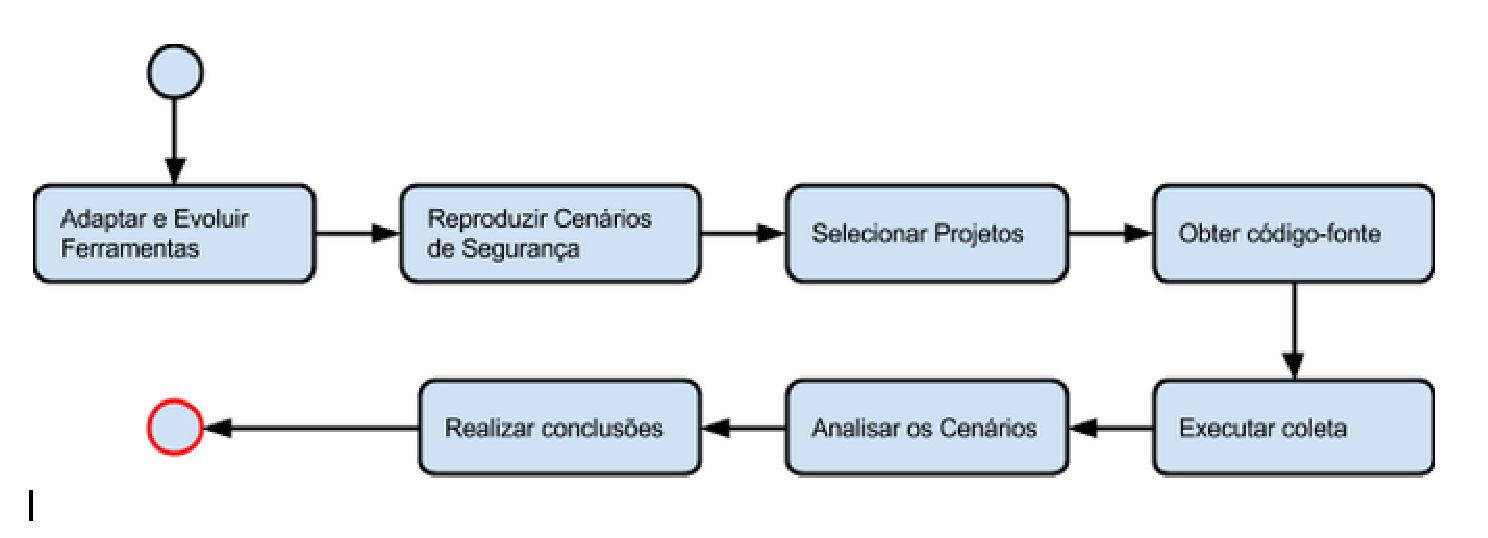
\includegraphics[width=1.0\textwidth]{fluxograma}
\caption{Método para execução dos estudos de casos.}
\label{method}
\end{figure}

Os passos da Figura~\ref{method} são melhor descritos a seguir:

\begin{enumerate}
\item \textbf{Adaptar e Evoluir Ferramentas} - Este passo consiste em evoluir as estruturas, modelos, componentes e camada de apresentação das ferramentas que serão utilizadas com o objetivo de melhor suportar a utilização de Cenários de Decisão.
\item \textbf{Reproduzir Cenários} - Uma vez que as ferramentas utilizadas já suportam a reprodução de Cenários, deve-se utilizar dessa estrutura para definir cenários reais para avaliação de projetos de software. No contexto dessa monografia, esse passo consiste em reproduzir os Cenários de Segurança criados no Mezuro e no \emph{DWing}.
\item \textbf{Selecionar Projetos} - Esta etapa consiste em definir quais projetos serão avaliados a partir dos cenários definidos e pode ser executada independente das ferramentas de tomada de decisão, variando de acordo com os objetivos de utilização dos Cenários.
\item \textbf{Obter Código-Fonte} - Uma vez selecionados os projetos, o próximo passo é obter o código-fonte referente aos projetos escolhidos. Algumas ferramentas. como o Mezuro, já possuem bom suporte para automatizar esse passo.
\item \textbf{Executar Coleta} - Esta etapa consiste na obtenção dos valores de métricas dos códigos-fontes dos projetos selecionados que deve ser automatizado. A saída desta etapa deverá ser processada pelas ferramentas trabalhadas para proporcionar a análise dos projetos. O esforço nessa etapa deve-se reduzir a coletar somente as métricas necessárias para composição dos Cenários de Decisão utilizados.
\item \textbf{Analisar Cenários} - A partir dos resultados obtidos, deve-se utilizar os Cenários de Decisão para observar as características do estado atual do projeto analisado. No contexto desse trabalho, esta etapa consiste em analisar quais os principais módulos oferecem riscos de segurança ao software. Porém, como o principal interesse é apresentar a utilização de cenários em ferramentas de tomada de decisões, esta etapa não será explorada detalhadamente.
\item \textbf{Realizar Conclusões} - Esta etapa final consiste em realizar ações a partir da compreensão dos Cenários observados, seja para fins de estudos ou para fins de desenvolvimento do software. 
\end{enumerate}


Estes passos metodológicos devem ser reproduzidos para cada ferramenta utilizada, sendo que uma vez que uma ferramenta já suporta adequadamente a observação de Cenários de Decisão, os passos 1 e 2 não precisam ser repetidos para análise de novos projetos.


\section{Cenários de Decisões no Mezuro}
\label{mezuro-cenarios}

O Mezuro é uma plataforma livre para monitoramento de código-fonte que busca auxiliar em vários problemas relacionados à utilização de métrica, visando ser uma interface que permita, de forma flexível, a extração e análise de métricas estáticas de código-fonte, licenciado como AGPLv3\footnote{\url{http://www.gnu.org/licenses/agpl-3.0.html}} \cite{manzo2014}. O Mezuro é uma plataforma concebida através do amadurecimento de diversas ferramentas, inicializada através do projeto Qualipso\footnote{Quality Platform for Open Source: \url{http://qualipso.icmc.usp.br/}}. Dentre estas ferramentas, destaca-se o Analizo\footnote{\url{http://analizo.org/}}, uma das ferramentas utilizadas pelo Mezuro para extração de métricas de código-fonte em C/C++ e Java.

A arquitetura do Mezuro atual é composta por vários serviços. Essa arquitetura está evoluindo para uma arquitetura de composição de quatro serviços principais que se resumem em:

\begin{itemize}
\item \textbf{Prezento}: Camada de apresentação da plataforma, desenvolvida em Ruby on Rails.

\item \textbf{Kalibro Gatekeeper}: Serviço que faz a intermediação e orquestração das outras camadas com o Prezento.

\item \textbf{Kalibro Processor}: Serviço que centraliza o processamento de métricas de projetos.

\item \textbf{Kalibro Configuration}: Serviço responsável pelo processamento de configurações.
\end{itemize}

Uma explicação mais detalhada desta arquitetura e de cada serviço pode ser obtida no Apêndice \ref{Att:mezuro}.

Dois destes serviços agregam conceitos fundamentais dentro da plataforma, que também serão muito importantes para a representação de cenários. 

O Kalibro Configuration contempla o conceito de configuração que é um conjunto de métricas e parâmetros que podem ser utilizadas para a avaliação de um projeto. Uma configuração consiste, portanto, na composição de métricas cujos valores de referência são flexíveis e podem ser determinados separadamente para cada configuração criada. Associado ao conceito de configuração, está a criação de intervalos qualitativos associado a valores de métricas. Este módulo ainda é complementado por \emph{Reading Gropus} que são grupos de leituras definidos por usuários que associam nomes qualitativos à cores que podem ser utilizados em configurações a partir na definição de intervalos de valores. Esta característica é muito importante para a utilização das métricas, uma vez que abstraem a interpretação direta dos valores obtidos para definições mais simples como bom, regular e ruim. Assim, tem-se a flexibilidade de ter parâmetros que variam de acordo com a linguagem, natureza do software, dentre outras coisas, apenas pela criação de diferentes configurações. 

O Kalibro Processor contempla o módulo de extração e processamento de métricas de código-fonte. Para que esse processamento seja realizado, o Kalibro Processor realiza o download de projetos que estão em repositórios GIT ou SVN e utiliza uma ou mais ferramentas de extração de métricas, como mencionado anteriormente. Assim, obtem-se a partir da análise estática do código-fonte um conjunto de métricas nativas que podem ser compostas para formular métricas mais complexas e de maior valor interpretativo. Dentro do Mezuro, esta abordagem é realizada através da criação de métricas compostas as quais serão muito importantes para a definição de Cenários de Decisões. 

Atualmente, o Mezuro pode monitorar projetos em C, C++ e Java uma vez que utiliza o Analizo como seu principal extrator de métricas. Entretanto, com a evolução da plataforma, pretende-se acoplar novos extratores na ferramenta para outras linguagens de programação.

Descrevemos a seguir os passos necessários para a utilização de Cenários de Decisões no Mezuro referente a realização das etapas Adaptar e Evoluir Ferramentas  e Reproduzir Cenários do estudo de caso. Todas as etapas exigem que haja um usuário autenticado no sistema.

\subsection{Criação do \emph{Reading Group} para os Cenários}

A criação de um \emph{Reading Group} para abstrair a interpretação do cenário é o primeiro passo para adaptação de cenários na ferramenta. Portanto, foi criado um grupo\footnote{\url{http://mezuro.org/reading_groups}} que define duas opções para a leitura de resultados binários, a fim de mostrar se existe ou não um cenário, usando a cor verde para a resposta falsa e vermelho para a resposta verdadeira. Este grupo é criado independente de configurações ou projetos dentro do Mezuro, de tal forma que pode ser utilizado por qualquer configuração que venha a reproduzir cenários. O grupo criado pode ser visto na Figura \ref{reading_group}.

\graphicspath{{figuras/}}
\begin{figure}[h]
\centering
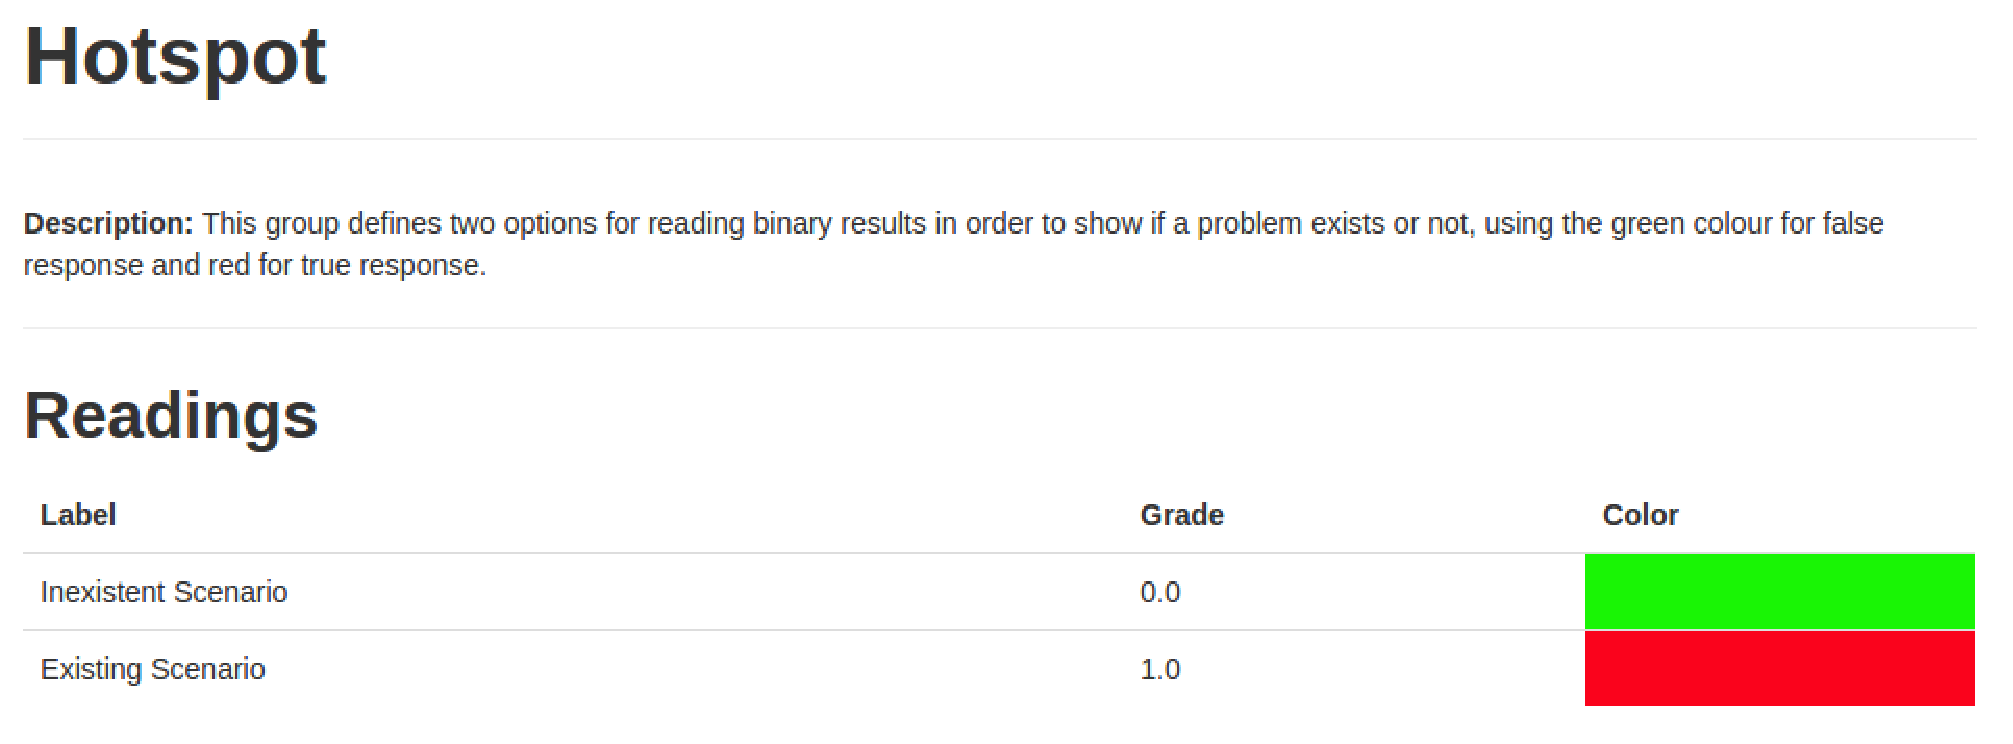
\includegraphics[width=1.0\textwidth]{reading_group}
\caption{Reading Group criado para Cenários. Disponível no Mezuro.org \url{http://mezuro.org/reading_groups/7}}
\label{reading_group}
\end{figure}

\subsection{Criação de uma Configuração para uma Categoria de Cenários}

Nesta etapa deve-se criar uma configuração onde serão definidos todos os cenários que queremos avaliar em conjunto. No contexto do Mezuro, os cenários serão definidos a partir do recurso de criação de Métricas Compostas que será explicado adiante.

Uma configuração, portanto, vai conter um conjunto de métricas e cenários caracterizados a partir dessas métricas. Como alternativas de criação de configurações como agregadores de cenários, teríamos a opção de criar uma única configuração que contemple todos os Cenários de Segurança que usam métricas de \emph{design} (\ref{cenarios-design}) e os Cenários de Segurança que usam métricas de vulnerabilidade (\ref{cenarios-vulnerabilidades}), da mesma forma que poderíamos criar uma configuração separada para cada tipo de cenário. O que mudaria é que, no primeiro caso o projeto seria monitorado uma única vez, enquanto no segundo o projeto deveria ser monitorado duas vezes, uma para cada configuração. 

Sugere-se que a segunda abordagem seja utilizada, pois flexibiliza mais o monitoramento a partir de cenários, uma vez que existem diversos projetos com diversos interesses diferentes. Além disso, vale ressaltar que uma configuração deve contemplar apenas uma linguagem de programação e domínio, uma vez que os parâmetros de avaliação dos Cenários irão variar de acordo com o contexto.

A criação de uma configuração é bem simples, pois deve-se informar apenas o nome e a descrição da configuração\footnote{\url{http://mezuro.org/mezuro_configurations}}. Assim, criou-se a configuração intitulada "Cenários de Decisões - Design Seguro para C++" para a categoria de cenários descrita em (\ref{cenarios-design}) como apresentado na Figura \ref{cenario_design}.

\graphicspath{{figuras/}}
\begin{figure}[h]
\centering
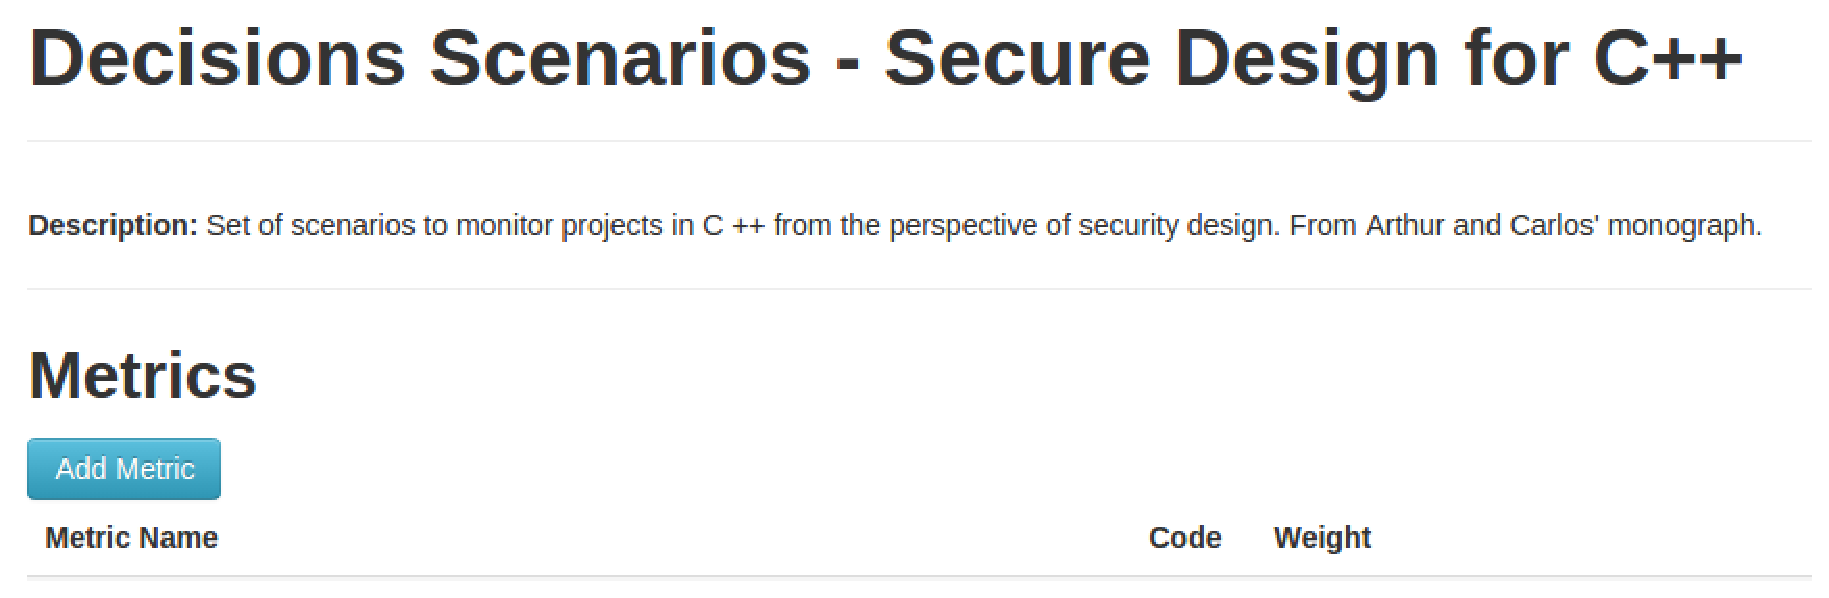
\includegraphics[width=1.0\textwidth]{cenario_design}
\caption{Configuração criada para Cenários de Design Seguro. Disponível no Mezuro.org \url{http://mezuro.org/mezuro_configurations/24}}
\label{cenario_design}
\end{figure}

Na visualização de uma configuração pode-se também ver a lista de métricas que compõem a configuração. Caso o usuário logado no Mezuro tenha a permissão  necessária de edição de uma determinada configuração, na tela de apresentação ainda pode ser vista a opção de Adicionar Métrica (\emph{Add Metric}), assim como apresentada na Figura \ref{cenario_design}. 

A opção de Adicionar Métrica é fundamental para a segunda etapa da criação da configuração. Portanto, após criada uma configuração, deve-se adicionar todas as métricas básicas que são utilizadas nas caracterizações dos cenários que irão compor essa configuração. Para isso, basta ir em \emph{Add Metric} na página da configuração, onde será aberta a lista de ferramentas coletoras utilizadas pelo Mezuro e as respectivas métricas suportadas por cada uma dessas ferramentas. 

No contexto da configuração criada para esta monografia foram adicionadas todas as métricas envolvidas nos Cenários de Decisões listados em (\ref{cenarios-design}). Todas as métricas escolhidas utilizam o Analizo como ferramenta extratora. A própria definição da métrica escolhida a partir de uma ferramenta também já define o escopo da métrica e as linguagens de programação para as quais a métrica pode ser calculada, conforme demonstrado na Figura \ref{metric_example}.

\graphicspath{{figuras/}}
\begin{figure}[h]
\centering
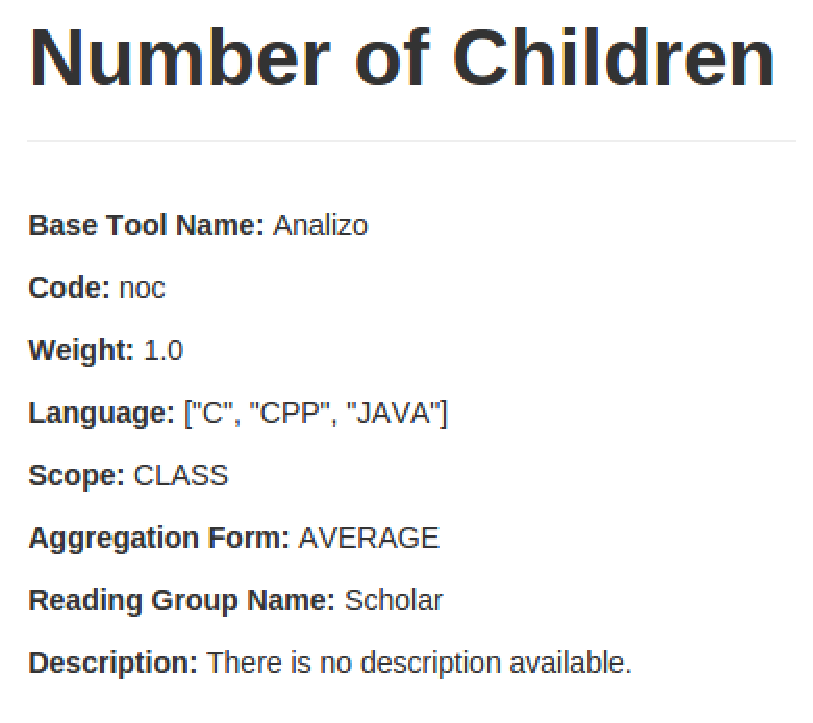
\includegraphics[width=0.5\textwidth]{metric_example}
\caption{Visualização da Métrica NOC no Mezuro. Disponível no Mezuro.org \url{http://mezuro.org/mezuro_configurations/24/metric_configurations/69}}
\label{metric_example}
\end{figure}

Como pode ser visto na Figura \ref{metric_example}, para cada métrica selecionada deve-se ainda definir o peso da métrica dentro da configuração (campo \emph{Weight}) e a forma de agregação da métrica (campo \emph{Aggregation Form}), que são informações importantes para a visualização da métrica em níveis de abstração maiores, principalmente a nível de pacotes e módulos. Para o contexto deste trabalho, mantivemos os valores 1.0 e Média para essas informações, tendo em vista que não são tão importantes neste caso, pois queremos observar nosso software principalmente a partir dos cenários, sendo os valores das métricas secundários, a serem utilizados somente por aqueles que desejam se aprofundar na caracterização dos cenários. Pelo mesmo motivo, não é necessário definir os intervalos para avaliação qualitativa dessas métricas básicas.

\subsection{Criação de Cenários}

Uma vez criada a configuração que irá conter os cenários e já adicionadas todas as métricas necessárias, o próximo passo é a criação dos Cenários de Decisões. Nesta etapa foi preciso estudos e evoluções sobre o Mezuro para determinar qual a melhor forma de representação dos cenários. Poderia-se adotar a estratégia de desenvolver uma estrutura de cenários novas, mas a partir da interação com a comunidade de desenvolvedores do Mezuro, optou-se por utilizar e evoluir o recurso de \textbf{métricas compostas}.

Dentro da ferramenta, métricas compostas são métricas que podem ser criadas a partir da composição das métricas bases das ferramentas extratoras adicionadas à uma configuração. Esta funcionalidade é muito interessante uma vez que flexibiliza a extensão da utilização do Mezuro para análise mais complexas que envolvem a composição matemática de outras métricas que não são diretamente extraídas dos projetos. Muitos estudos científicos apresentados ao longo desta monografia propõem novas métricas a partir da composição de métricas básicas conhecidas.

Para a definição de como a métrica composta deve ser calculada, o usuário deve escrever um \emph{script} simples em Javascript que retorne o valor desejado. Como é definido um identificador para cada métrica básica adicionada na configuração (campo \emph{Code} visível na Figura \ref{metric_example}), nos \emph{scripts} para métricas compostas pode-se acessar os valores das métricas extraídas a partir de uma chamada de método cujo nome é o mesmo do código da métrica. Para exemplo, dentro do \emph{script} poderia-se acessar o valor da métrica \emph{Number of Children} através da chamada \emph{noc()}, onde \emph{noc} é o código dessa métrica.

Além da utilização de \emph{scripts}, assim como as métricas básicas, as métricas compostas ainda possuem informações de nome e descrição que são essenciais para a definição do quadro resumo do cenário. A utilização de heranças e polimorfismo relacionados às métricas no \emph{design} do Mezuro são muito importantes para a extensão de outros tipos de métricas. Neste sentido, algumas contribuições foram realizadas ao serviço Prezento relacionadas à refatorações que apoiam a extensão de outros tipos de métricas. 

No futuro, com a adoção de novos extratores na plataforma e novas métricas, será necessário o estabelecimento de um novo tipo de métrica (\emph{hot spot}) cuja natureza não está na quantificação e sim na existência ou não de determinada característica no código-fonte. Exemplos desse novo tipo de métrica são métricas de vulnerabilidade e até mesmo os Cenários de Decisões. Entretanto, como dito anteriormente, optou-se por utilização de métricas compostas para a definição dos cenários e não na criação de um novo tipo de métrica.

Na maior parte dos casos de utilização de métricas compostas, os \emph{scripts} são simples e retornam apenas o resultado de uma operação matemática simples entre métricas e números. Entretanto, devido as características de definição dos cenários, principalmente dos cenários Polimétricos, deve-se utilizar outras estruturas nesses \emph{scripts} tal como estruturas condicionais.

Como mencionado anteriormente, os Cenários de Decisões possuem características de métricas \emph{hot spots} cujo valor medido é booleano baseado na existência ou não do cenário. Como ainda não há suporte a valores do tipo verdadeiro ou falso no Mezuro, os \emph{scripts} de Cenários devem retornar 1 no caso de existência do cenário e 0 no caso de não existência.

Em resumo, a criação da uma métrica composta para um Cenário de Decisão deve conter um script que siga uma estrutura semelhante à listada a seguir:

\begin{lstlisting}[caption={Estrutura de script básica para Cenários de Decisões}, label=script_example]
if(cenario_existente)
{
  return 1;
}
else
{
  return 0;
};
\end{lstlisting}

\subsection{Associando o \emph{Reading Group} ao Cenário}

\graphicspath{{figuras/}}
\begin{figure}[h]
\centering
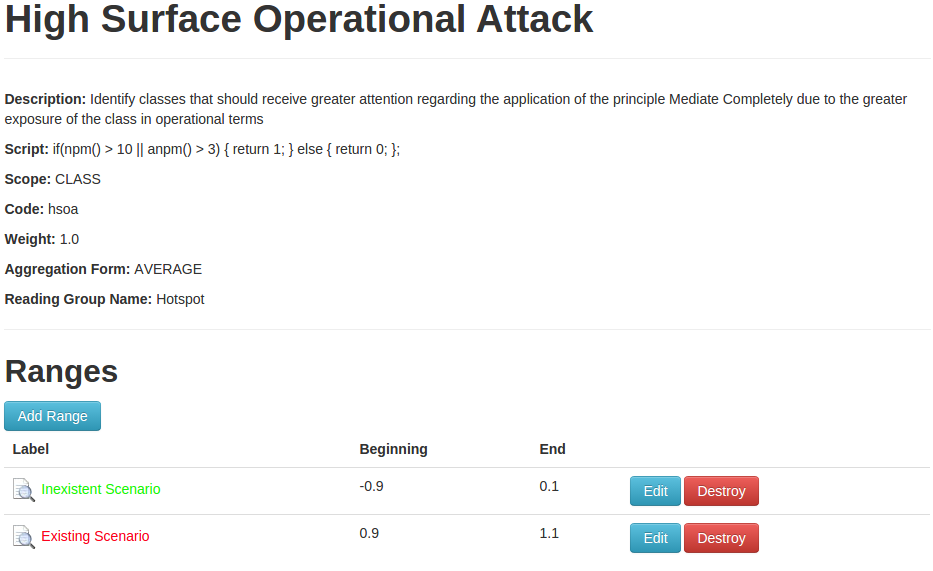
\includegraphics[width=1.0\textwidth]{cenario_completo}
\caption{Cenário Completo representado no Mezuro. Disponível no Mezuro.org \url{http://mezuro.org/mezuro_configurations/24/compound_metric_configurations/67}}
\label{cenario_completo}
\end{figure}

Após criada a métrica composta para um cenário, a última etapa que resta é associar os valores que podem ser obtidos pela métrica composta às interpretações qualitativas do \emph{Reading Group} criado na primeira etapa descrita na presente Seção. Portanto, associaremos os valor obtido 1 ao grupo \emph{Existint Scenario} (em vermelho) e o valor 0 ao grupo \emph{Inexistint Scenario} (em verde) que podem ser vistos na Figura \ref{reading_group}.

Para realizar esta etapa basta ir na visualização pública da métrica composta criada e adicionar dois intervalos, como mencionado. Como pode ser observado na Figura \ref{cenario_completo}, para o valor qualitativo \emph{Inexistint Scenario} definiu-se o valor -0.9 à 0.1, enquanto para o valor \emph{Existint Scenario} definiu-se o intervalo de 0.9 à 1.1. Essa definição de intervalos é necessária uma vez o Mezuro não suporta valores de métricas booleanos, conforme discutido anteriormente. A Figura \ref{cenario_completo} apresenta a visualização pública de um Cenário de Decisão criado através de uma métrica composta no Mezuro.

A seguir será apresentado os scripts utilizadas na criação de cada Cenário de Decisão de Design Seguro no Mezuro. Os códigos utilizados em chamadas de métodos representam as métricas básicas envolvidas no cenário, conforme explorado na explicação de cada cenário.

\begin{description}
	\item[Alta Superfície de Ataque a Atributos Internos]
\end{description}

\begin{lstlisting}[caption={\emph{Script} do Cenário \emph{High Surface Attack to Internal Attributes}}, label=hsaia]
if(noa() == 0) 
{
  return 0;
}
else
{
  var result = npa()/noa();
  var value = (result < 0.2) ? 0 : 1; 
  return value;
};
\end{lstlisting}

\begin{itemize}
	\item \textbf{npa} - Número de Atributos Públicos
	\item \textbf{noa} - Número de Atributos
\end{itemize}

\begin{description}
	\item[Alta Superfície de Ataque Operacional]
\end{description}

\begin{lstlisting}[caption={\emph{Script} do Cenário \emph{High Surface Operational Attack}}, label=hsoa]
if(npm() > 10 || anpm() > 3)
{
  return 1;
}
else
{
  return 0;
};
\end{lstlisting}

\begin{itemize}
	\item \textbf{npm} - Número de Métodos Públicos
	\item \textbf{anpm} - Média de Parâmetros por Método
\end{itemize}

\begin{description}
	\item[Ponto Crítico de Falha]
\end{description}

\begin{lstlisting}[caption={\emph{Script} do Cenário \emph{Critical Point of Failure}}, label=cpf]
if(acc() + noc() > 5)
{
  return 1;
}
else
{
  return 0;
};
\end{lstlisting}

\begin{itemize}
	\item \textbf{acc} - Número de Classes Aferentes
	\item \textbf{noc} - Número de Filhos
\end{itemize}

\begin{description}
	\item[Risco Elevado de Segurança]
\end{description}

\begin{lstlisting}[caption={\emph{Script} do Cenário \emph{High Risk Security}}, label=cpf]
if(accm() > 4 || amloc() > 10)
{
  return 1;
}
else
{
  return 0;
};
\end{lstlisting}

\begin{itemize}
	\item \textbf{accm} - Média de Complexidade Ciclomática por Método
	\item \textbf{amloc} - Média de Número de Linhas por Método
\end{itemize}

\section{Cenários de Decisão e \emph{Data Warehousing}}
\label{dw-cenarios}

\emph{Data Warehousing} (\emph{DWing}) é um ambiente constituído pelo \emph{Data Warehouse} (\emph{DW}) e as demais ferramentas relacionadas a manipulação de dados, desde a extração até a visualização. Um ambiente de \emph{DWing} não se diz respeito apenas das tecnologias envolvidas e sim uma arquitetura que requer o suporte de diferentes tipos de tecnologias \cite{inmon2002}.  As principais tecnologias envolvidas em um ambiente de \emph{DWing} são SGBDs, Sistemas de conversão e transformação de dados (ferramentas de ETL), tecnologias cliente e servidor para dar acesso aos dados a múltiplos clientes e ferramentas de análise e geração de relatórios.

Como o nome sugere, um \emph{Data Warehouse} , em português, significa armazém de dados. Segundo Inmon (\citeyear{inmon2002}) um \emph{Data Warehouse} é uma coleção de dados de uma corporação que tem como objetivo dar suporte a tomada de decisão. 
%
O DW possibilita a análise de grandes volumes de dados, fazendo com que ele seja o núcleo de muitas soluções de \emph{Business intelligence} (BI)
%
\footnote{\emph{Business intelligence} é o processo de coleta, organização, análise, compartilhamento e monitoramento de informações, oferecendo suporte a gestão de negócios}. 
%
Uma explicação mais detalhada sobre os  conceitos relacionados a um ambiente de \emph{DWing} pode ser obtida no  apêndice \ref{Att:dw}.

Neste trabalho procuramos desenvolver mecanismos que nos permitam monitorar e analisar o código fonte através de métricas de forma automatizada e que nos auxilie na tomada de decisão de refatorar ou não refatorar determinadas partes do código. 
%
Nesse sentido, foram encontrados alguns trabalhos na literatura que utilizaram um \emph{DWing} para monitorar métricas de processos e produtos de software \cite{Folleco2007} \cite{Silveira2010}\cite{mazuco2011} \cite{rego2014}. Dentre estes, o trabalho que se destaca e que serviu como ponto de partida para a criação do modelo dimensional do DW desta monografia foi o trabalho de Rego (\citeyear{rego2014}). Nele, o autor propõe um \emph{DWing} que além de monitorar métricas de um projeto,  identifica e monitora cenários de limpeza de código fonte compostos por métricas relacionados a qualidade de software.

% 
O fato de o DW oferecer um alto poder de análise e permitir o tratamento de uma grande quantidade de dados nos faz ter uma expectativa de que esse ambiente pode ser uma solução mais completa em termos de monitoramento e auxílio na tomada de decisão. 

Nesta Seção, apresentamos a execução das etapas Adaptar e Evoluir Ferramentas e Reproduzir Cenários de Segurança para o estudo de caso sobre o ambiente \emph{DWing}.

\subsection{Modelagem Dimensional}

A modelagem dimensional é uma técnica de modelagem de banco de dados para auxílio a consultas do DW. Ela é de grande importância, se não a principal etapa de desenvolvimento de um ambiente de \emph{DWing}, pois é nessa etapa que os requisitos de negócio são traduzidos em um modelo de dados que permitirá realizar as consultas desejadas. Uma boa modelagem irá permitir um bom desempenho, intuitividade e escalabilidade de um DW.

%
Antes partirmos para modelagem de nosso DW,  precisamos ter definidas as necessidades do negócio. No caso dessa monografia, queremos conseguir monitorar e visualizar quais os cenários estão ocorrendo no projeto e também monitorar o valor de suas métricas que estão envolvidas nos cenários, de modo que, ao identificar que um determinado cenário está acontecendo, seja possível também identificar as métricas que estão relacionadas com a ocorrência do cenário, ajudando assim a identificar quais ações devemos tomar para solucionar essa ocorrência. Também queremos observar esses cenários ao longo do tempo, permitindo a realização de análises por \emph{sprint}, mês, etc. Dessa forma, temos dois fatos claros: (1) um fato para registrar a quantidade de cenários e (2) outro para registrar o valor das métricas.

 \begin{figure}[H]
 	\centering
 		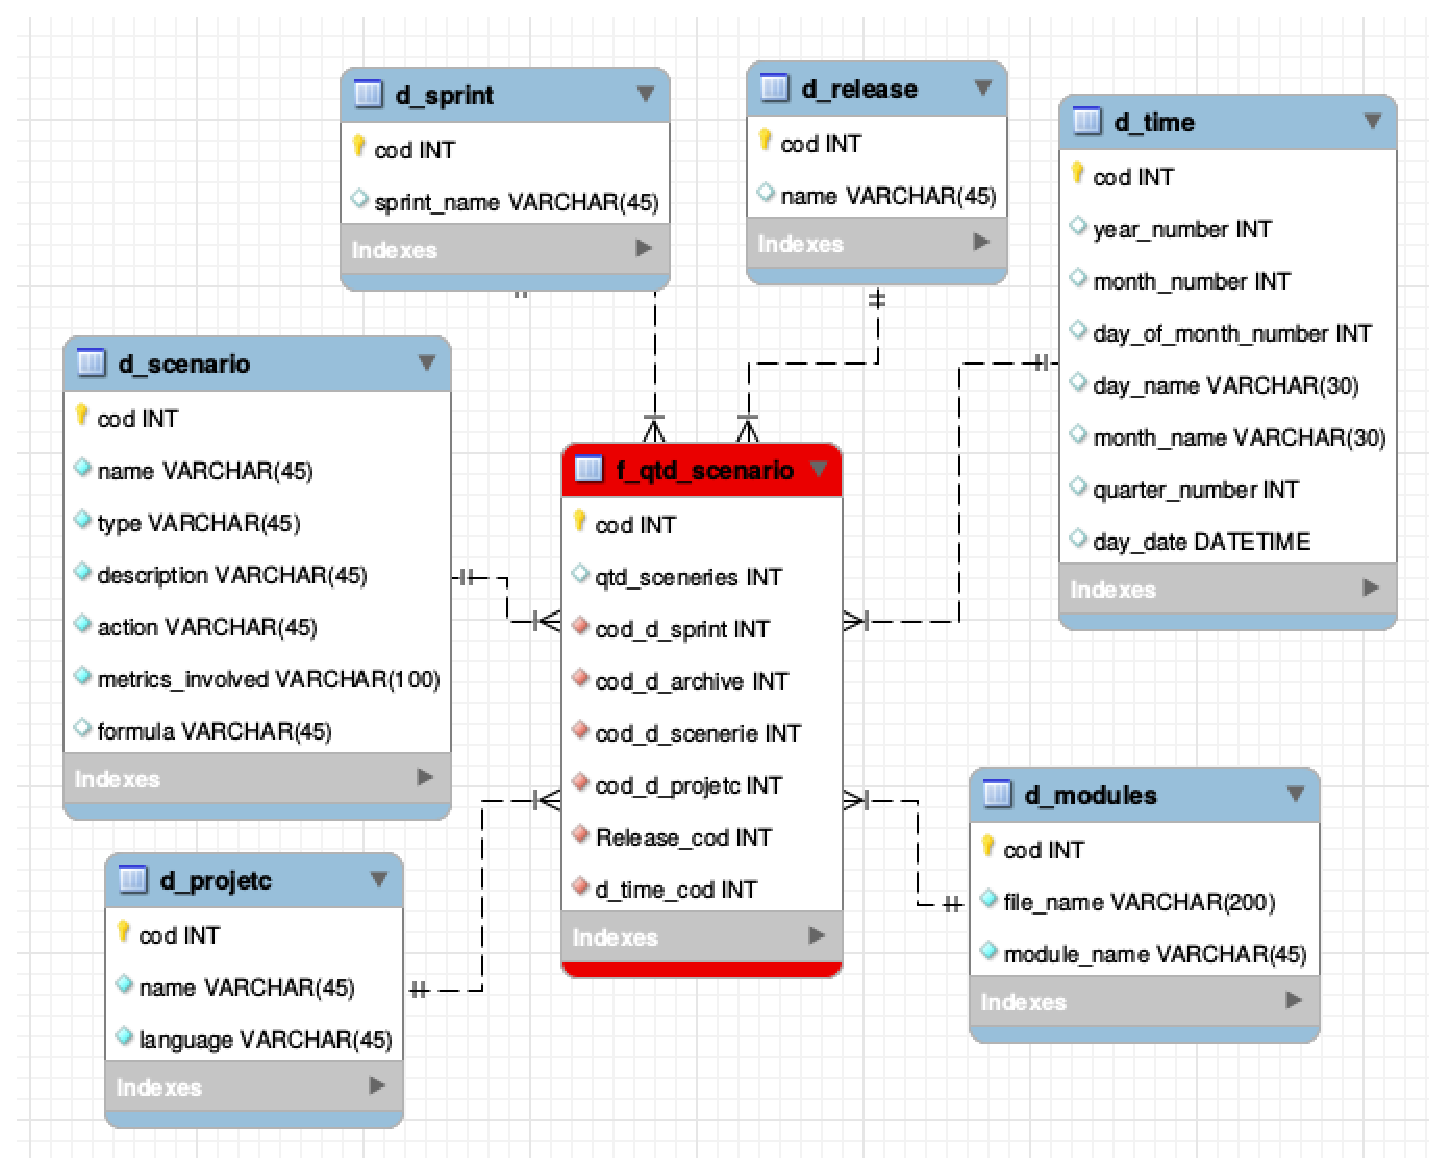
\includegraphics[scale=0.5]{figuras/dw-f-scenarios}
 		\caption{Modelo dimensional do fato \emph{f\_qtd\_scenarios} que irá armazenar os cenários identificados no projeto.}
 		\label{dw-model1}
 \end{figure}

 

 \begin{figure}[H]
 	\centering
 		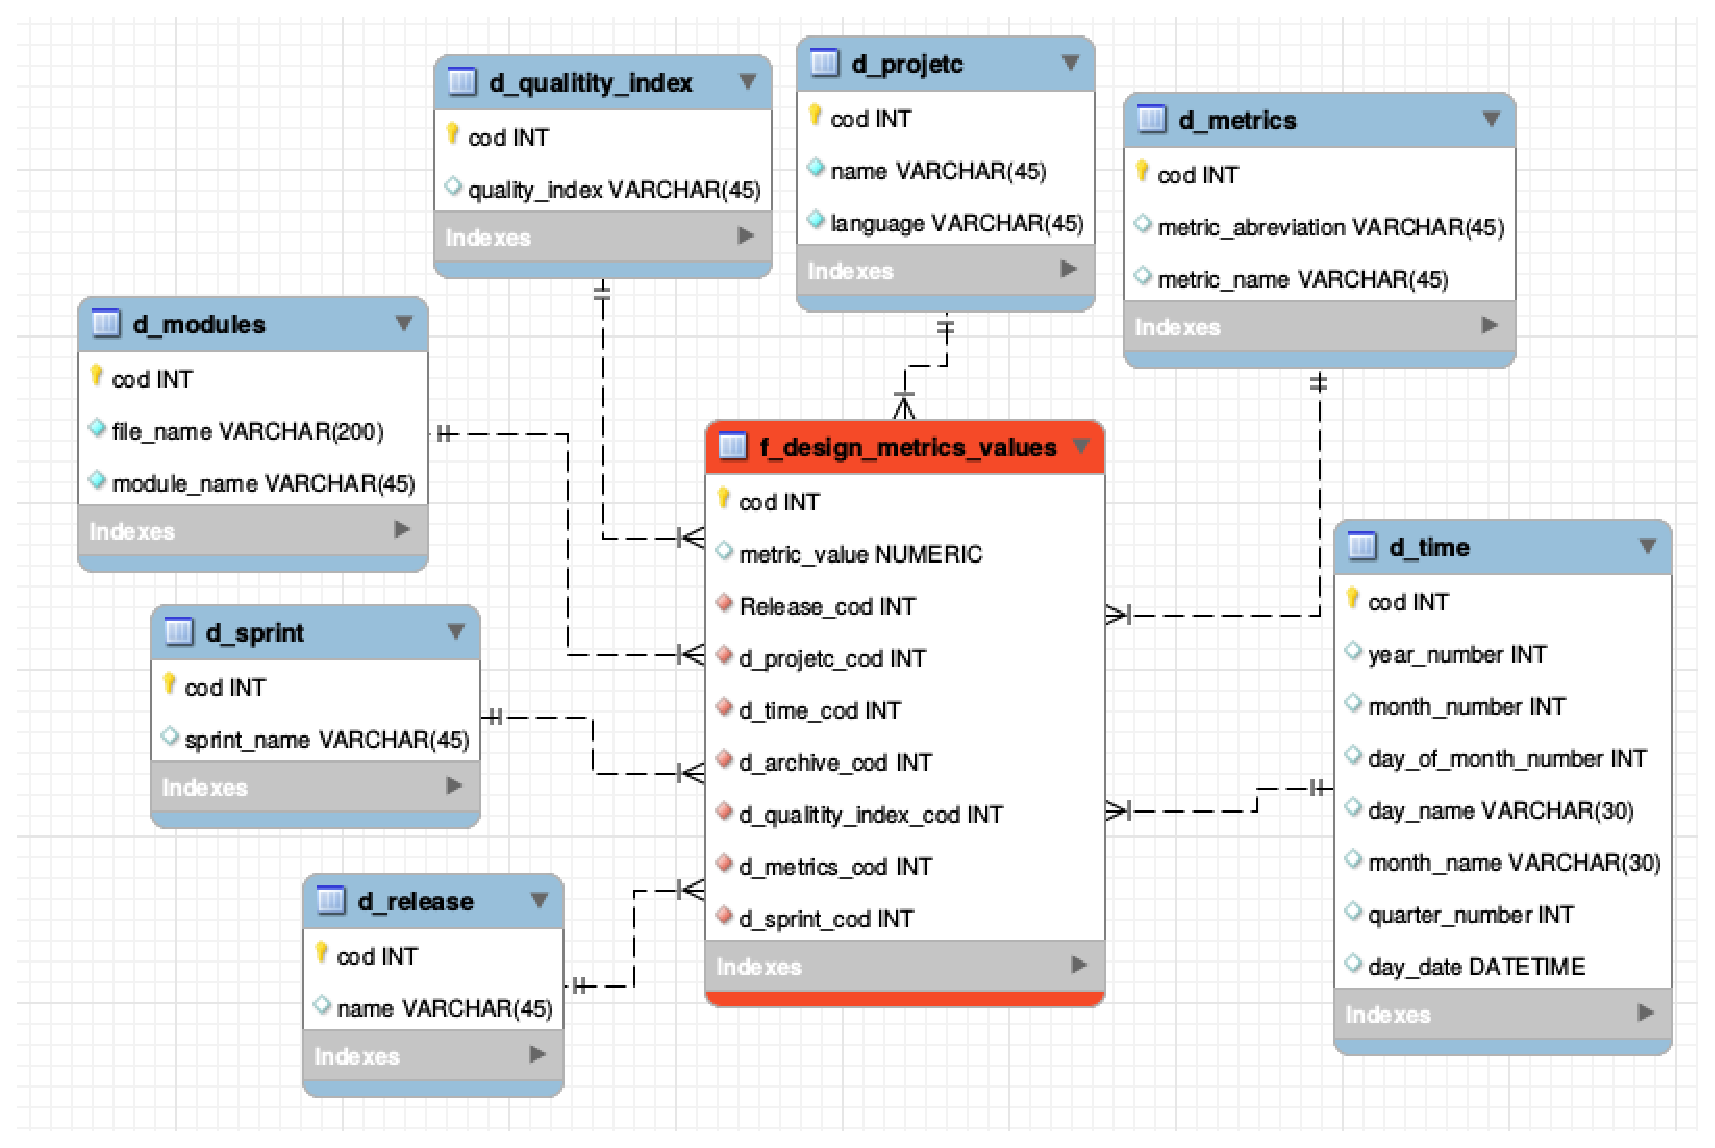
\includegraphics[scale=0.5]{figuras/dw-fato-design-metrics}
 		\caption{Modelo dimensional do fato \emph{f\_design\_metrics\_values} que irá armazenar os valores das métricas de cada classe do projeto.}
 		\label{dw-model2}
 \end{figure}

 

 \begin{figure}[H]
 	\centering
 		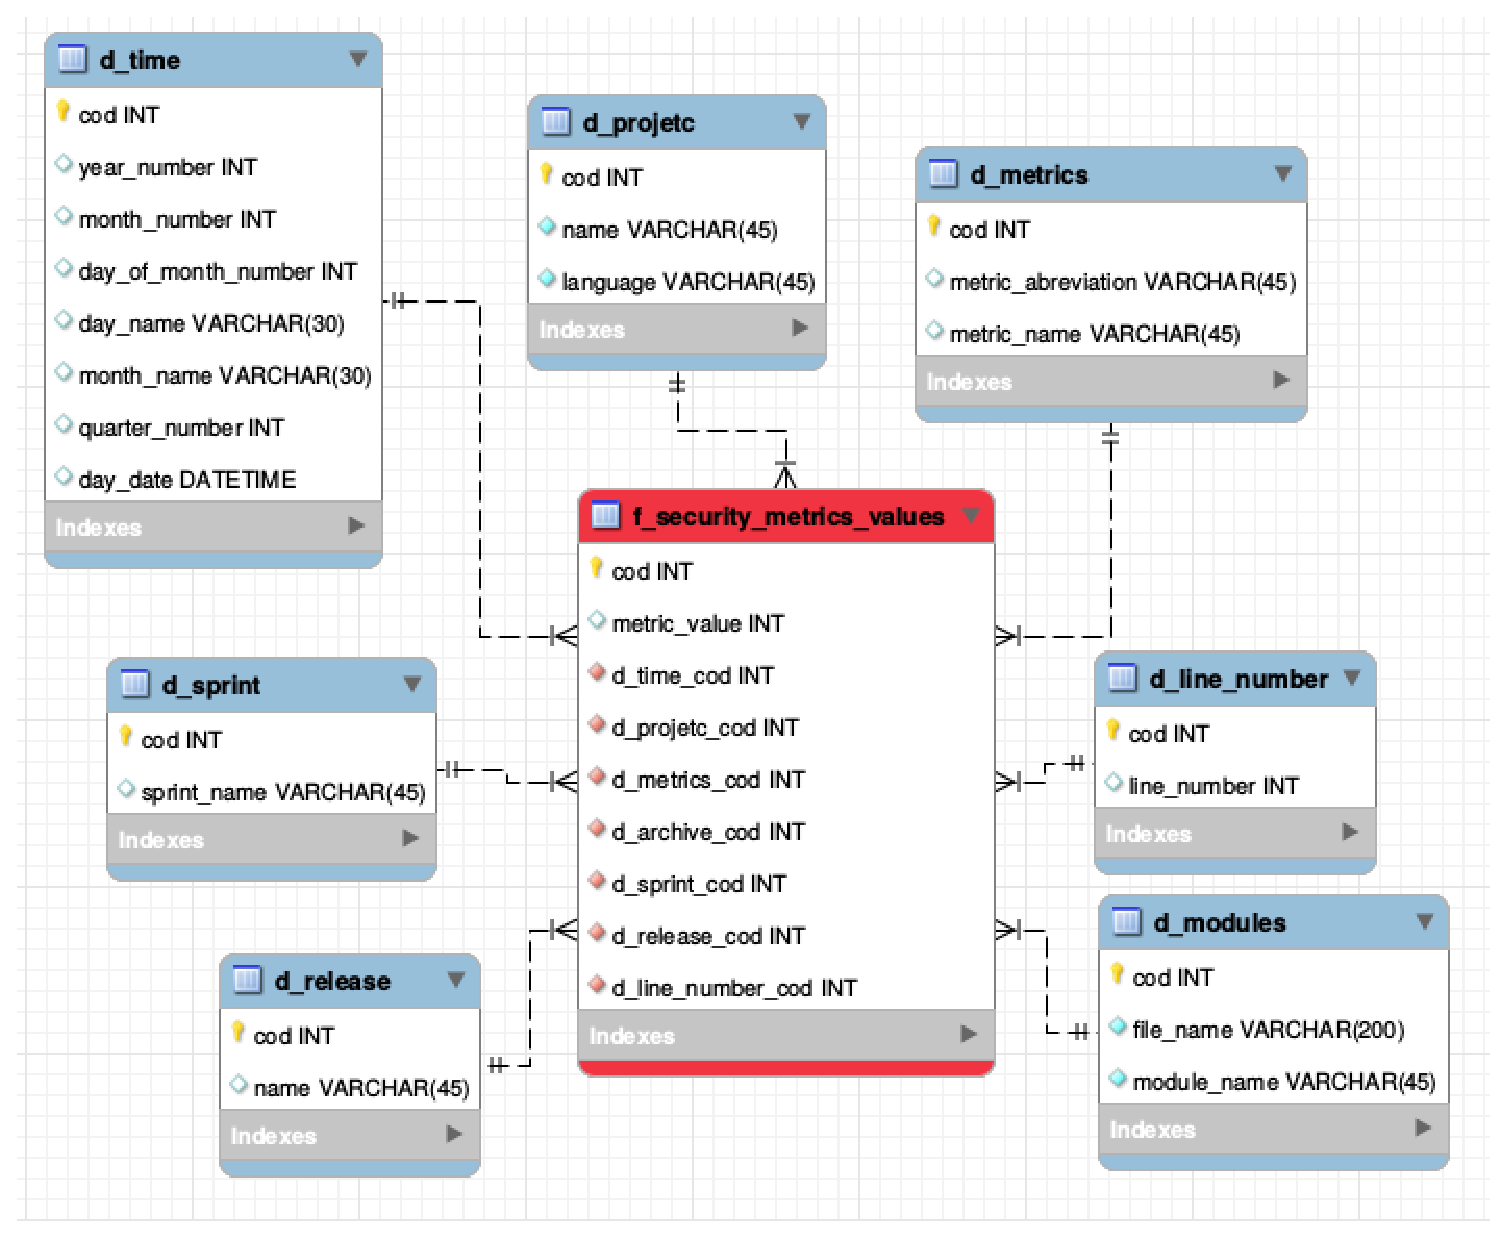
\includegraphics[scale=0.5]{figuras/dw-fato-security-metrics}
 		\caption{Modelo dimensional do fato \emph{f\_security\_metrics\_values} que irá armazenar os valores das métricas de segurança de cada arquivo do projeto.}
 		\label{dw-model3}
 \end{figure}


No trabalho de Rego \citeyear{rego2014} observamos que a modelagem proposta pelo autor está próxima de atender as necessidades dessa monografia. A modelagem de Rego \citeyear{rego2014} permite que o usuário possa identificar cenários de limpeza ao nível de classe de código fonte e também monitorar os percentis dos valores de métricas \emph{design} do projeto. Baseado nisso, chegamos na modelagem mostrada nas Figuras (\ref{dw-model1}) (\ref{dw-model2}) e (\ref{dw-model3}) para o DW deste trabalho.

Alguns aspectos da modelagem do trabalho de Rego (\citeyear{rego2014}) foram modificados e evoluídos para atender melhor a definição dos cenários de decisões proposta nessa monografia. A tabela fato de cenários (\emph{f\_qtd\_scenarios}) que pode ser vista na Figura \ref{dw-model1}  foi modelada de maneira muito semelhante. Porém, foram adicionadas a dimensão tempo e de \emph{sprints}. Uma das principais características de um ambiente de \emph{DWing} é permitir a análise temporal dos dados, logo viu-se interessante a inclusão da dimensão tempo. Da mesma forma, a dimensão \emph{sprint} permitirá o usuário a fazer análise da quantidade de cenários por \emph{sprint}. 

Outra modificação importante foi feita na dimensão \emph{d\_scenarios}. Novos atributos foram incluídos para contemplar a estrutura de cenários de decisões proposta nessa monografia. Foram inclusos os atributos tipo do cenário, métricas envolvidas, fórmula e uma descrição. Uma limitação do trabalho de Rego (\citeyear{rego2014}) foi que os cenários só podiam ser compostos por no máximo duas métricas. Isso se dá ao fato de que Rego utilizou  metadados para definir quais métricas estavam envolvidas a cada cenário e automatizar de maneira mais eficiente a identificação de novos cenários. Neste trabalho, levamos em conta que  metadados não são disponibilizados para o usuário, preferimos criar o atributo \emph{involved\_metrics} e \emph{formula} na dimensão \emph{d\_scenario}, permitindo assim que o usuário possa saber quais métricas compõe cada cenário e como elas definem a existência ou não do cenário. Como se trata de um atributo de natureza descritiva, podemos ter cenários que possuem várias métricas envolvidas.

Rego também criou outro fato para armazenar os valores percentis das métricas de um determinado projeto. Para este trabalho, achamos que seria melhor o fato relacionado aos valores das métricas ser a nível de módulo. Dessa forma, o usuário tem mais insumo para identificar a causa de um cenário em uma classe específica. Por exemplo, suponhamos que o usuário tenha identificado a ocorrência do cenário \emph{Ponto crítico de falha} em uma determinada classe. Posteriormente, o usuário pode verificar qual foi o valor das métricas ACC e NOC nesse módulo e tomar uma decisão de refatoração baseado nos valores dessas métricas. No trabalho de Rego (\citeyear{rego2014}), como os valores das métricas estariam disponíveis ao nível de projeto apenas, esse tipo de análise não poderia ser feito.

Em nossa modelagem, preferimos separar em duas tabelas fatos as métricas de \emph{design} e as métricas de segurança. A motivação foi que esses dois tipos de métricas possuem natureza diferente. Métricas de vulnerabilidade contam o número de ocorrência de uma determinada vulnerabilidade no código. Logo, podemos realizar agregações e descobrir a quantidade de vulnerabilidade do mesmo tipo por arquivo, por projeto, etc. Já com métricas de \emph{design}, nem sempre é possível fazer esse tipo de agregação de somatório com seus valores. Outro aspecto desses dois fatos é que, como discutido no Capítulo \ref{cap-cenarios}, não temos um índice de qualidade para métricas de vulnerabilidade, tornando essa dimensão inutilizada na fato \emph{f\_security\_metrics\_values}. Por outro lado, é possível chegar ao nível de linha para caracterizar uma vulnerabilidade, incluindo então a dimensão \emph{d\_line\_number} a esse fato.



\subsection{Criação do ambiente de \emph{DWing}}

O ambiente de \emph{DWing} foi criado conforme a Figura \ref{dw_components}.

 \begin{figure}[H]
 	\centering
 		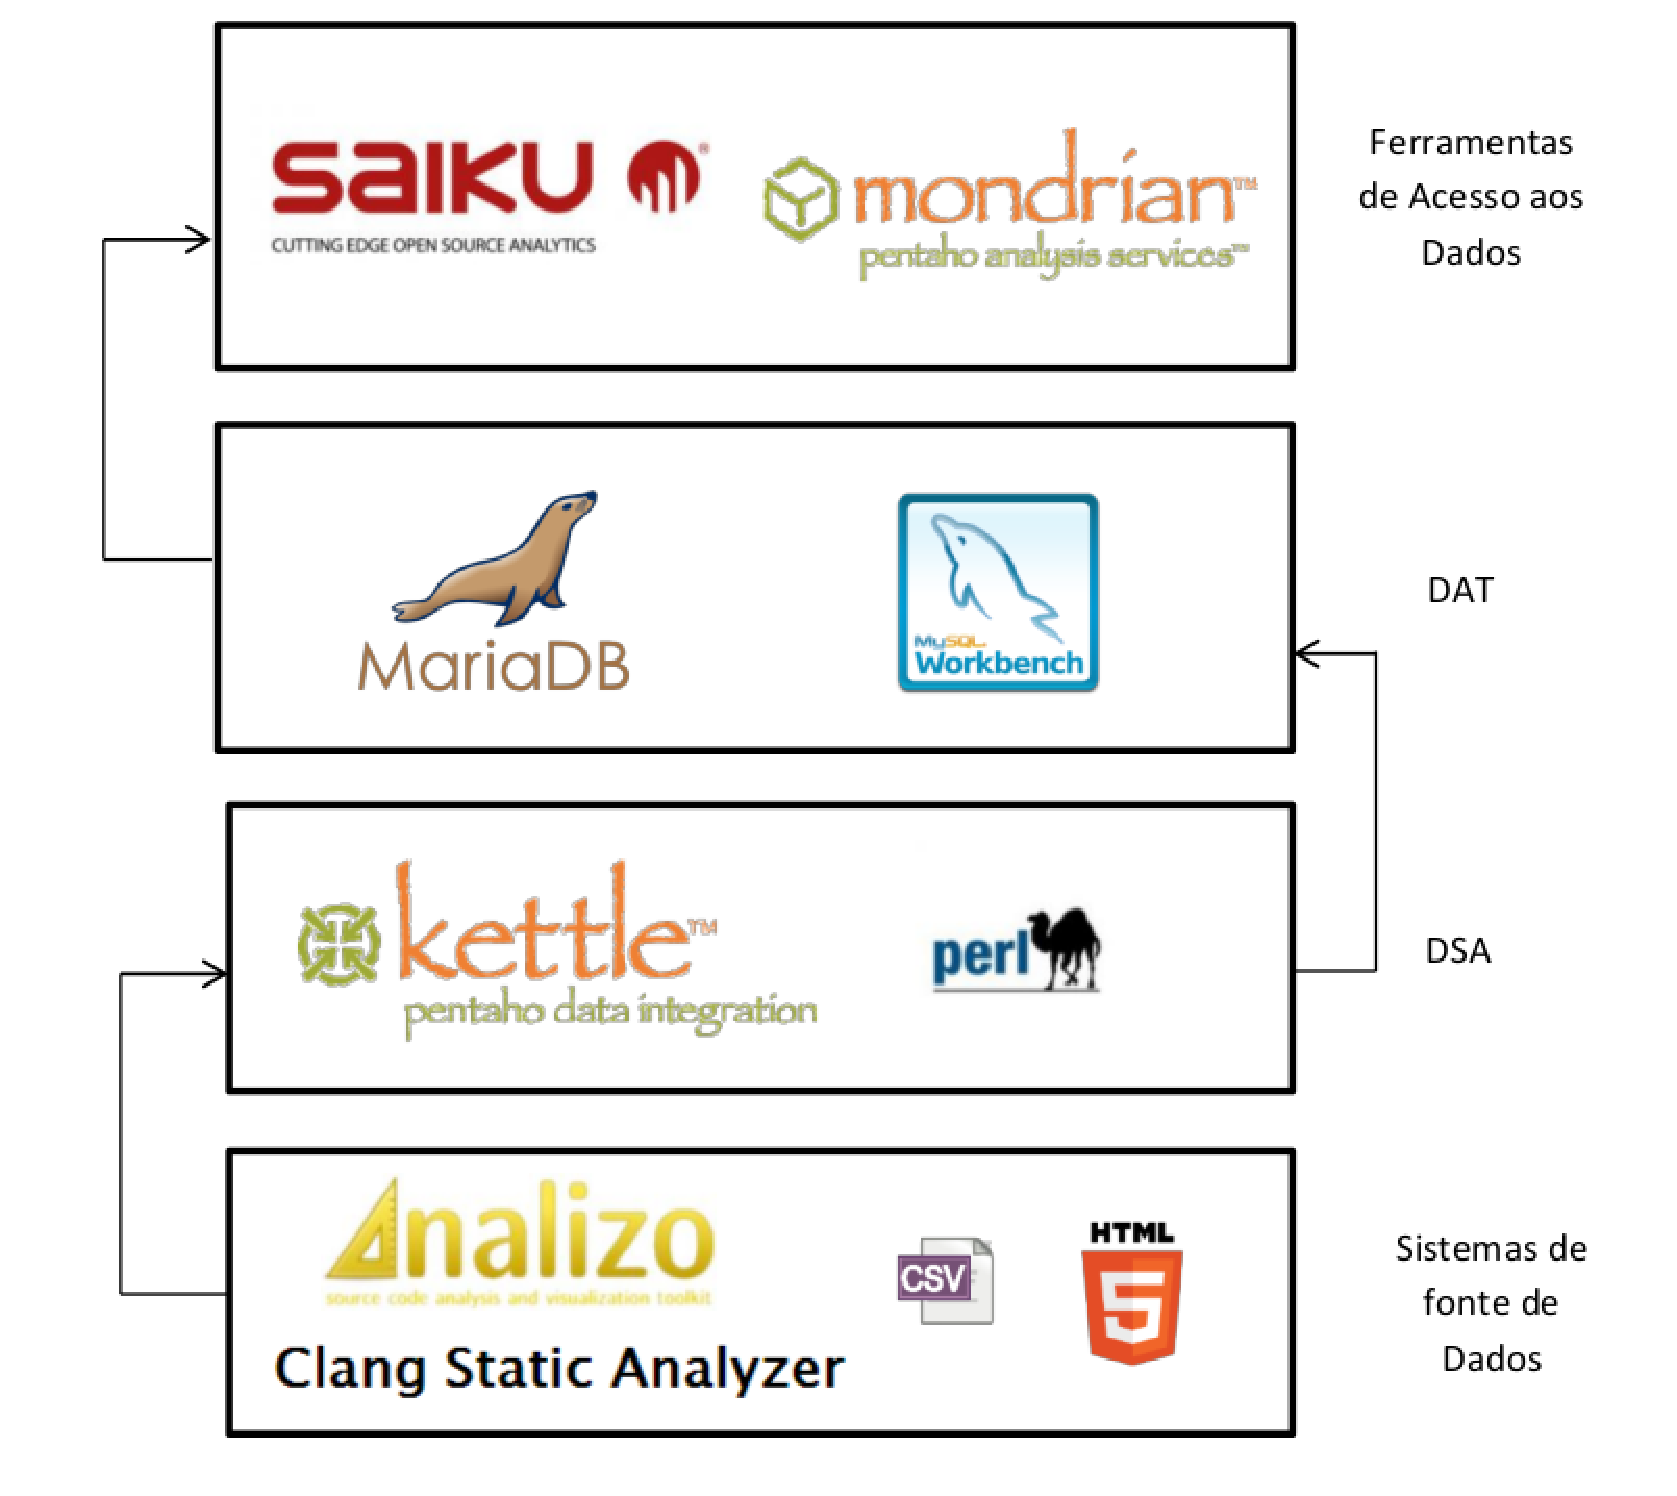
\includegraphics[scale=0.5]{figuras/dw_components}
 		\caption{Ferramentas utilizadas para o desenvolvimento do ambiente de \emph{DWing}.}
 		\label{dw_components}
 \end{figure}


Como podemos ver na Figura \ref{dw_components}, as métricas foram coletadas do Analizo e do \emph{Clang static Analyzer}. O uso do Analizo por si só deveria ser o suficiente, pois este oferece valores de métricas tando de design quanto de vulnerabilidade. Porém, foi identificado um problema com o Analizo que não consegue gerar métricas de vulnerabilidade para projetos maiores. Esse problema será melhor explicado mais adiante na Seção (\ref{data-colect}). Dessa forma, foi utilizado o \emph{Clang-Static-Analyzer}\footnote{\url{http://clang-analyzer.llvm.org/}} para coletar apenas as métricas de vulnerabilidades.

%
Os dados são disponibilizados na forma de arquivos CSV, por parte do Analizo, e HTML, por parte do clang. Porém, a fim de facilitar a extração desses dados, foi criado um parser para transformar esse relatório HTML para um arquivo CSV de estrutura parecida com o relatório do Analizo.


Para o processo de ETL foi utilizado uma ferramenta da suíte de ferramentas Pentaho, chamada de \emph{Pentaho Data Integration}\footnote{\url{http://community.pentaho.com/projects/data-integration/}} (PDI). O PDI aceita diversos formatos de entrada de Dados, além de fazer integração com diversos banco de dados, incluindo o MariaDB \footnote{\url{https://mariadb.org/pt-br/}}, que foi o SGBD utilizado para a implementação do DW. É no processo de ETL que são identificados os cenários de decisão. Diferente do Mezuro, que são feitas configurações na própria ferramenta para que ela possa identificar os cenários de decisão, no \emph{DWing} o processo de ETL já identifica o cenário e já passa a informação pronta para ser a armazenada do \emph{Data Warehouse} (qual a classe, release, projeto, entre outros atributos que estão envolvidos com a identificação daquele cenário).

\begin{landscape}

\begin{figure}[H]
 	\centering
 		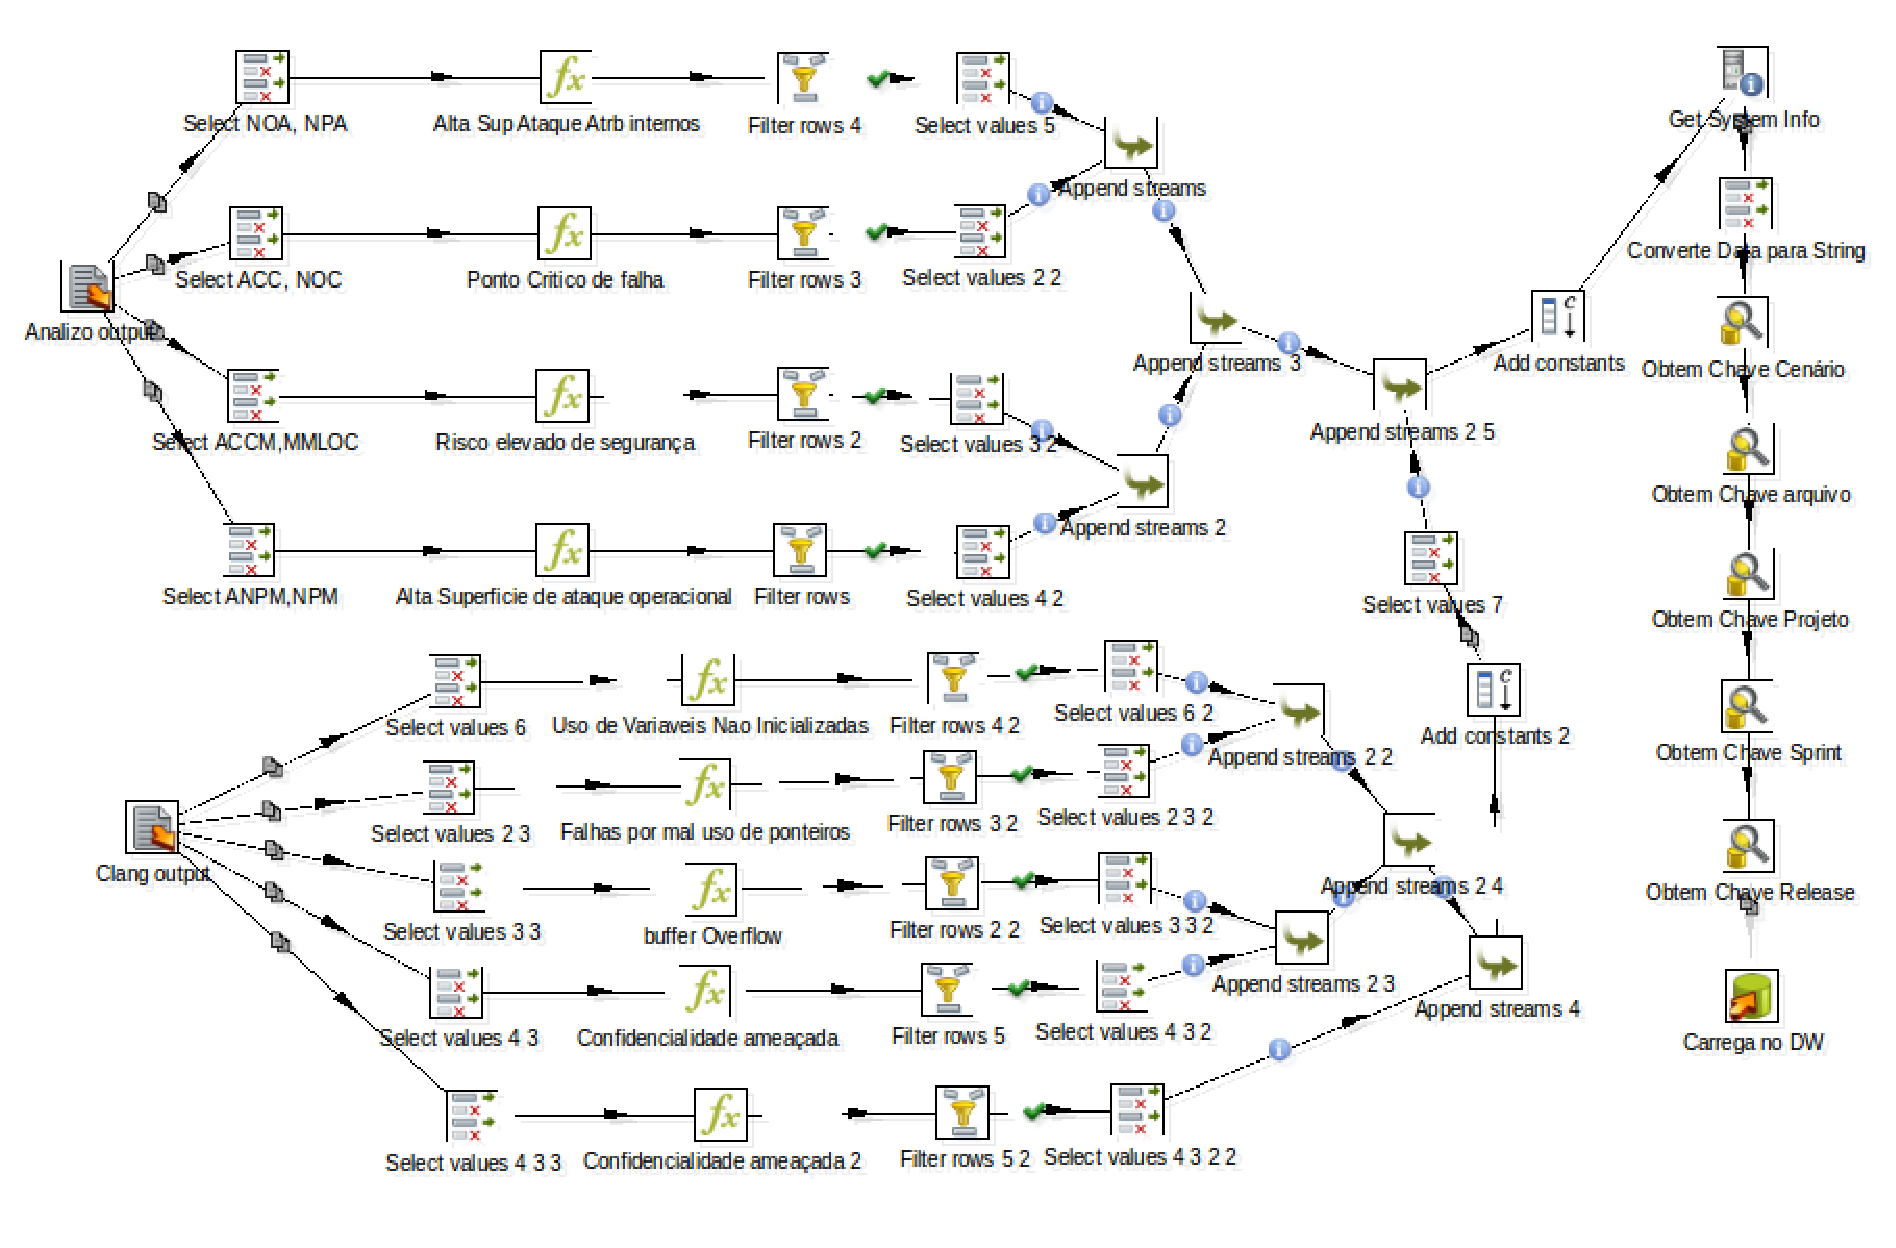
\includegraphics[scale=0.7]{figuras/dw-etlpdi}
 		\caption{Processo de ETL para identificação dos cenários de decisão feito no PDI}
 		\label{dw-etl-pdi}
 \end{figure}

\end{landscape}
Na Figura \ref{dw-etl-pdi} é demonstrado o processo de ETL, elaborado na ferramenta PDI através de uma \emph{transformation}, responsável por extrair os dados, identificar os cenários e carregar a informação no DW. De maneira resumida, os dados são extraídos de arquivos CSV. Esses dados contém informações a respeito das classes e arquivos, e o valor das diversas métricas suportadas pelas ferramentas para cada classe. Para cada cenário, são selecionadas apenas as métricas de interesse para então verificar se o cenário existe o não em determinada classe. É no step \emph{formula} (steps caracterizados pelo \emph{Fx}) onde colocamos a regra de identificação do cenário. Dessa forma, quando o cenário é identificado, este é atribuído a aquela classe. Nos passo posteriores os dados são limpos e preparados até formarem uma tupla que será carregada na tabela de fatos.


Os processos de ETL para carregar os fatos relacionados aos valores das métricas foram mais simples, pois consistiu basicamente em armazenar o relatório fornecido pelas ferramentas. Apenas as métricas que compõe os cenários criados foram selecionadas para serem armazenadas do DW.


Os dados são armazenados no \emph{Data Warehouse}, implementado em um banco de dados MariaDB. Foi utilizado o \emph{MySql Workbench}\footnote{\url{http://www.mysql.com/products/workbench/}} para criação dos modelos e das tabelas.


Para visualizar os dados, realizar consultas OLAP e gerar relatórios, foi utilizado a ferramenta \emph{Pentaho Business Inteligence Server}\footnote{\url{http://community.pentaho.com/}} (conhecida como BI server). Essa ferramenta ainda inclui a tecnologia de cliente e servidor, possibilitando o acesso de diversos usuários a um sistema de consultas e análise em rede. Ela conta com diversos plugins que realizam diversas operações, tais como, geração de gráficos, visualização de dados em tabelas, etc. O Plugin utilizado para a visualização dos dados e geração de consultas OLAP foi o \emph{Saiku Analytics}\footnote{\url{http://www.meteorite.bi/}}.

Entretanto, antes de visualizar os dados, é necessário primeiramente criar cubos de dados. Para criação e publicação do cubos de dados, foi utilizado a ferramenta Mondrian \footnote{\url{http://sourceforge.net/projects/mondrian/files/schema\%20workbench/}}. Esta gera um arquivo XML com todas as configurações definidas do cubo, que é usado pelo BI \emph{server} para gerar os relatórios e fazer as conultas OLAP à base de dados. É nessa etapa onde definimos quais são as hierarquias e agregações que poderão ser feitas em cima dos dados no momento das análise.



\section{Projetos analisados}
\label{cap-projects}

Nesta monografia definimos a técnica de Cenários de Decisão e propomos um conjunto de cenários para tomada de decisão sobre a segurança do software, seja a partir da utilização de métricas de \emph{design} ou através de métricas de vulnerabilidades. Para apresentar como estes cenários podem ser utilizados, foram utilizados três softwares livres cujos resultados do monitoramento irão ser utilizados para demonstrar a visualização dos cenários.

Como discutido no Seção \ref{cap-cenarios-sec-definicaocenarios} do Capítulo de Cenários, nos restringimos a apenas projetos escritos em C++. A seguir é feita uma pequena introdução à cada um dos projetos escolhidos.

\subsection{GNU Octave}
\label{section-octave}

O GNU Octave é um projeto desenvolvido em C++ que consiste em uma linguagem interpretada de alto nível destinada à computação matemática distribuída através da licença GNU General Public License \footnote{\url{http://www.gnu.org/copyleft/gpl.html}}. Ele possui uma interface baseada em linha de comando para a solução de problemas matemáticas lineares e não lineares, assim como possibilita a execução de experimentos numéricos. Além disso, também provê um conjunto extensivo de ferramentas para geração de gráficos, visualização e manipulação de dados.

Outras informações específicas sobre o projeto GNU Octave podem ser obtidas através da documentação oficial do projeto, disponível na página \url{https://www.gnu.org/software/octave/}.

O código fonte do projeto está disponível na página \url{ftp://ftp.gnu.org/gnu/octave}. Lá, além da versão atual, podemos ter acesso ao código de releases anteriores.

Este projeto será analisado tanto através do Mezuro quanto através do DWing.


\subsection{Athom Shell}
\label{section-athom}

O Athom Shell é um framework desenvolvido em C++ que permite escrever aplicações \emph{desktop} multi-plataforma através de JavaScript, HTML e CSS. Esse framework é baseado em node.js\footnote{\url{http://nodejs.org/}} e no Chromium e é usada no editor de texto Athom\footnote{\url{https://atom.io/}}. Esse projeto é distribuído através da licença MIT\footnote{\url{http://opensource.org/licenses/MIT}}.

A documentação oficial do projeto pode ser encontrada no próprio repositório principal\footnote{\url{https://github.com/atom/atom-shell}} através da url: \url{https://github.com/atom/atom-shell/tree/master/docs}.

Avaliação através do Mezuro pode ser vista em: \url{http://mezuro.org/projects/33/repositories/58}

\subsection{Synergy}
\label{section-synergy}

O Synergy é um programa escrito em C++ que permite compartilhamento de mouse e teclado entre computadores que não necessariamente utilizam o mesmo sistema operacional. Além disso permite copiar e colar conteúdos de um sistema operacional para outro. Esse projeto é distribuído através da licença GNU General Public License \footnote{\url{http://www.gnu.org/copyleft/gpl.html}} e possui uma wiki bem completa, indicando até padrões de codificação seguidos no projeto.

A documentação oficial pode ser encontrada em sua wiki através da url: \url{http://synergy-project.org/wiki/Main_Page}

Este projeto será analisado somente no \emph{DWing}.

\section{Coleta de Dados}
\label{data-colect}

O Mezuro já trabalha em conjunto com o Analizo\footnote{\url{http://www.analizo.org/}}. O Analizo é uma ferramenta de análise estática de código e dá suporte a diversas métricas, inclusive as métricas discutidas no capitulo 2, tanto de \emph{design} quanto de vulnerabilidade. Um \emph{DWing} não está atrelado a apenas uma fonte de dados, podendo utilizar diversas fontes. Dessa forma, utilizamos o Analizo para coletar as métricas e gerar o insumo para a análise dos cenários em ambas as soluções.

Porém, foi identificado um problema com o Analizo em relação as coleta de métricas de vulnerabilidade. Para projetos pequenos e simples as métricas de vulnerabilidade podem ser coletadas.  Contudo, para projetos maiores e mais complexos, com arquitetura bem definida, o Analizo não consegue gerar tais métricas. Isso se deve ao fato do Analizo utilizar o \emph{Clang Static Analizer}\footnote{\url{http://clang-analyzer.llvm.org/}}, que é outra ferramenta livre que faz análise estática para identificação de bugs em projetos C/C++, para a geração das métricas de vulnerabilidade. A utilização do \emph{Clang} consiste em chamar o comando \emph{scan-build}  e o comando de compilação do programa, por exemplo " \emph{scan-build gcc myprog.c} ". O Analizo chama o \emph{clang} em seu código para cada arquivo, usando apenas o comando  de compilação \emph{gcc} em cada um deles. Isso pode funcionar para projetos simples, porém projetos mais complexos possuem linhas de compilação mais complexas, geralmente gerenciadas em um \emph{Makefile}, com diversas linhas de compilação. Não conseguindo compilar o código, o \emph{Clang} não consegue executar, fazendo com que o Analizo, por sua vez, não consiga extrair as métricas de vulnerabilidade. 

Grandes alterações deveriam ser feitas para que o Analizo pudesse gerar os valores dessas métricas para projetos grandes, não cabendo ao escopo e tempo desta monografia. Esse problema afeta diretamente ao Mezuro, pois, dependente do relatório gerado pelo Analizo, não consegue os valores de métricas de vulnerabilidade para projetos maiores. Como o ambiente de \emph{DWing} pode ter diversas fontes de dados, podemos recorrer a outra fonte de dados que ofereça apenas as métricas de vulnerabilidade.

Dessa forma, decidimos usar o próprio  \emph{clang} para extrair as métricas de vulnerabilidade. O \emph{clang} gera um relatório no formato HTML. Foi feito um parser para transformar o HTML em um arquivo CSV, com a mesma estrutura fornecida pelo Analizo. Assim, o ambiente de \emph{DWing} pode utilizar desse arquivo CSV gerado pelo parser para se alimentar das métricas de vulnerabilidade da mesma maneira que trata o CSV gerado pelo próprio Analizo. O parser foi desenvolvido na linguagem perl justamente para aproveitarmos das lógicas de programação e códigos do próprio Analizo responsáveis pela geração do CSV.

No Mezuro, para se analisar um projeto, deve-se criar um projeto informando o seu nome e descrição\footnote{\url{http://mezuro.org/projects}}. Para cada projeto pode-se fazer diferentes análises, utilizando diferentes configurações, através da criação de Repositórios dentro do Mezuro onde devem ser informados o nome, descrição, a licença, tecnologia de versionamento utilizada, o endereço para o repositório e a configuração desejada. Além disso, o Mezuro possui um recurso interessante para acompanhamento de projetos: a definição da periodicidade para coletas periódicas que varia desde periodicidade diária à mensal, sendo este um recurso opcional.

Uma vez salvo um repositório com a devida configuração e endereço para o repositório, o Mezuro realiza o download do projeto e, através do Kalibro Processor, executa os extratores envolvidos na configuração utilizada sobre o projeto. Assim, o relatório gerado pelas ferramentas são tratados e enviados de volta para o Prezento, onde são apresentados os resultados das medições. Caso a opção de coleta periódica seja utilizada, o Mezuro irá sempre fazer o download da versão mais recente.


No \emph{DWing}, uma vez criado o mecanismo de ETL, utilizando a ferramenta PDI, basta selecionarmos os arquivos  CSV  quem contém os relatórios da versão do código que se deseja analisar. A seleção dos arquivos CSV são feitas nos steps \emph{Analizo output} e \emph{Clang output}, que podem ser visualizados na Figura \ref{dw-etl-pdi}. O ambiente de \emph{DWing} não permitiu, como no Mezuro, a automatização completa, desde a coleta até a geração das análises. No \emph{DWing} temos que ter os relatórios das ferramentas (Analizo e Clang) em mãos, para então carregar os dados e gerar as análises. Entretanto, é possível automatizar todo esse processo com o auxílio de shellscripts e utilização de Jobs\footnote{Assim como as \emph{Transformations}, os \emph{Jobs} são um tipo de componente do PDI que possibilita executar tarefas de mais alto nível, como mandar e-mails, baixar arquivos, executar transformações, etc} no PDI, mas tais atividades não couberam nos escopo deste trabalho.


\section{Análise dos Cenários nas Ferramentas}

Nesta Seção será apresentada a visualização dos cenários nas duas ferramentas apresentadas através do monitoramento dos projetos apresentados na Seção \ref{cap-projects}.

O projeto GNU Octave foi monitorado através do Mezuro e do ambiente DWing. O projeto Athom Shell foi analisado somente através do Mezuro, enquanto o projeto Synergy foi monitorado somente através do ambiente DWing.

\subsection{Visualização no Mezuro}
\label{vision-mezuro}

A visualização de qualquer monitoramento realizado no Mezuro segue uma apresentação semelhante. Primeiro são apresentadas as informações do projeto, seguido das informações sobre o \emph{status} do monitoramento e data de realização (Figura \ref{proc_info}). Logo após é apresentada uma árvore contendo os módulos e classes do projeto e o resultado agregado das métricas medidas  (Figura \ref{modules_info}). A medida que se realiza uma navegação sobre a árvore de módulos, diminui-se a granularidade dos resultados e tem-se os resultados das medições para cada unidade de software analisada (Figura \ref{metrics_info}).

Caso algum erro ocorre durante o processo de medição, o erro será informado na aba \emph{Processing information}, apresentada na Figura \ref{proc_info}. 

\begin{figure}[H]
	\centering
		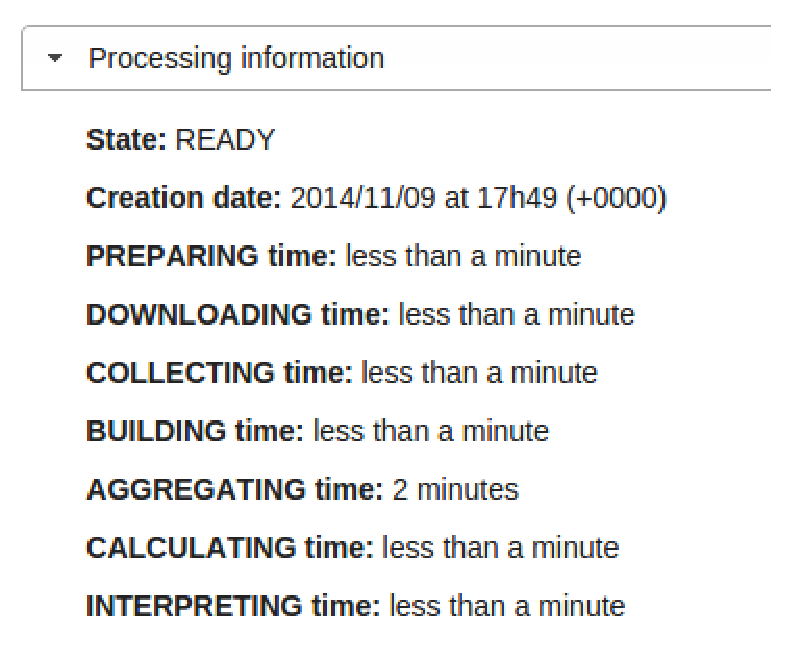
\includegraphics[scale=0.5]{figuras/proc_info}
		\caption{Apresentação do processo de coleta de métricas no Mezuro}
		\label{proc_info}
\end{figure}

A segunda aba \emph{Modules Tree}, destacada na Figura \ref{modules_info}, apresenta todos os módulos encontrados no projeto e seus respectivos níveis de granularidade. Cada item apresentado é um link para o respectivo módulo, onde são apresentados somente os sub-módulos e as medições daquele módulo. Portanto, a navegação entre os módulos e os resultados individuais de cada módulo é bem simples dentro da plataforma, permitindo uma análise detalhada e aprofundada.

\begin{figure}
	\centering
		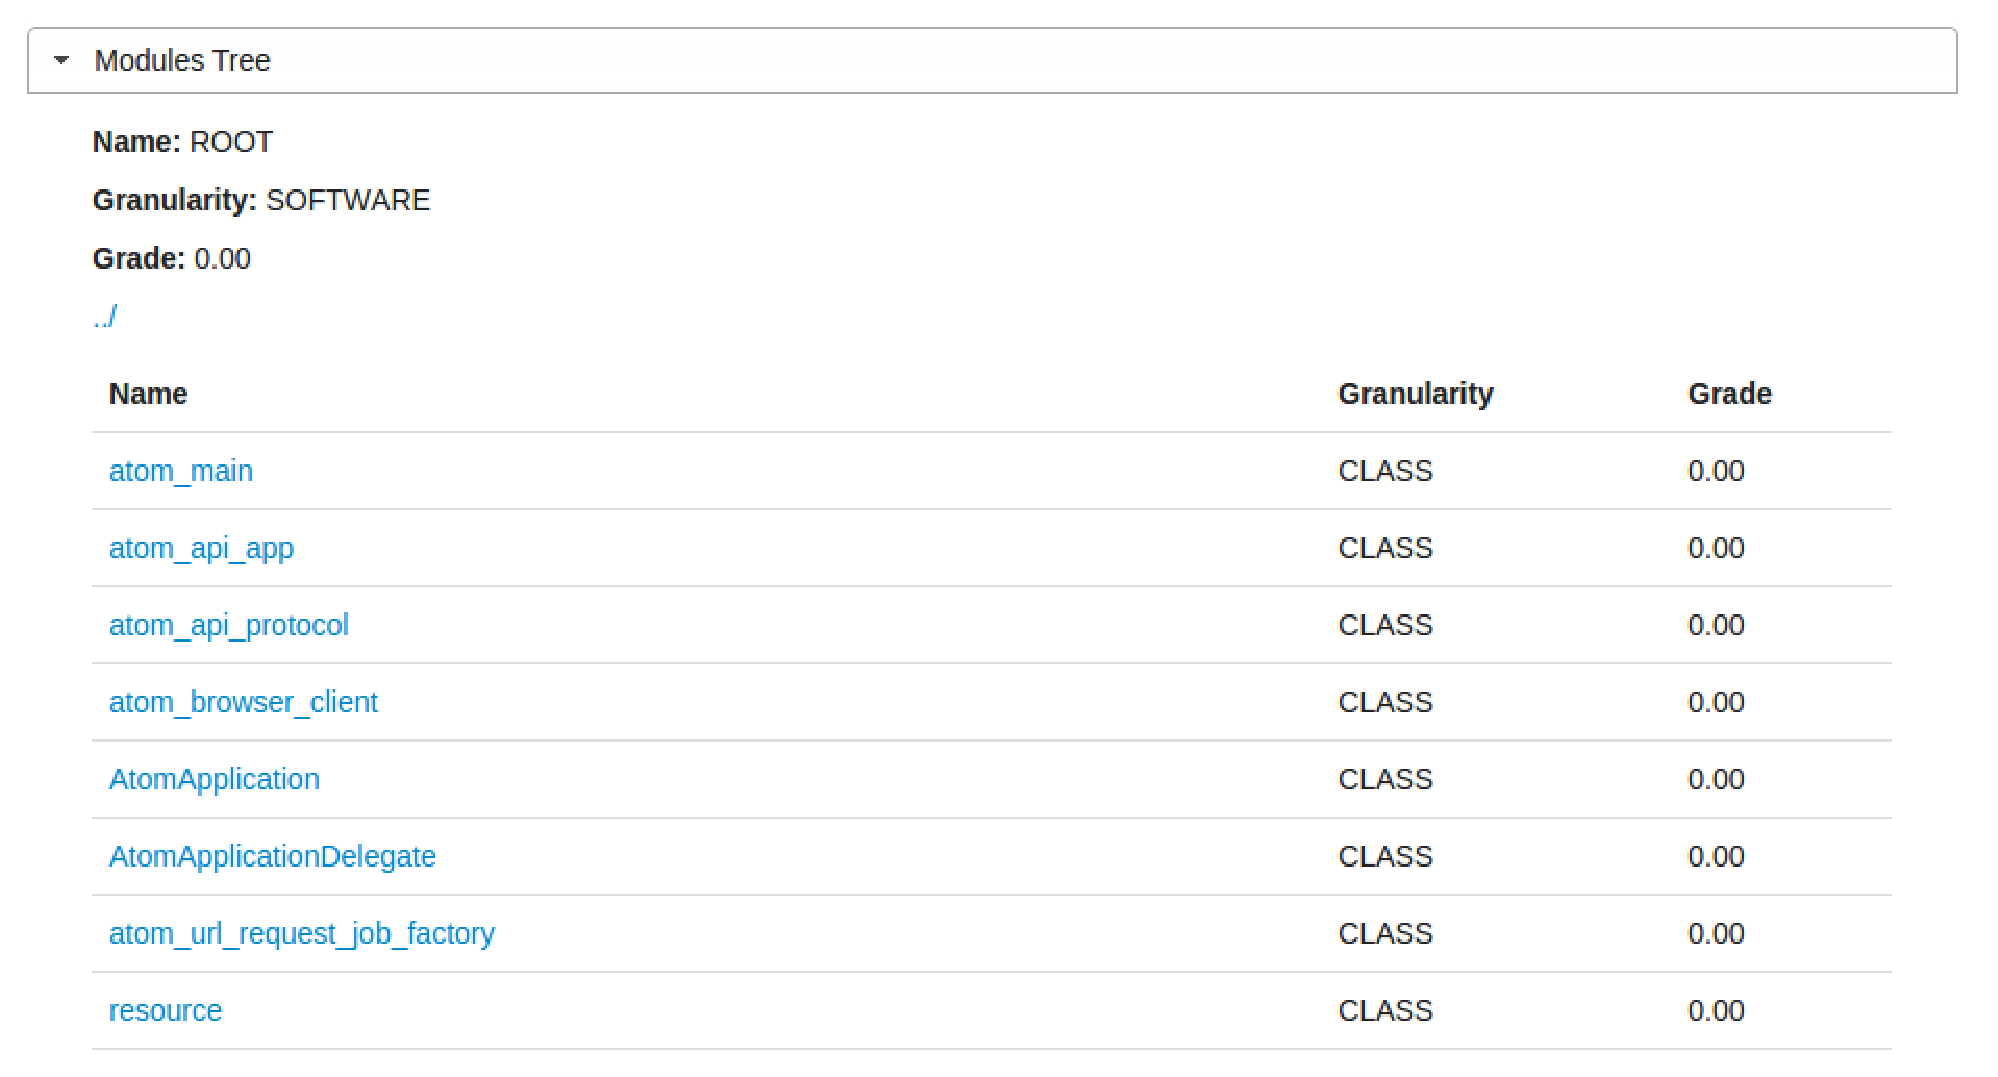
\includegraphics[scale=0.5]{figuras/modules_info}
		\caption{Apresentação da árvore de módulos do Mezuro}
		\label{modules_info}
\end{figure}

A última aba \emph{Metrics Results}, apresentada na Figura \ref{metrics_info}, lista as métricas básicas medidas e as métricas compostas, com seus resultados agregados, no caso de visualização de pacotes, ou com seus resultados medidos, no caso de visualização de unidades ou classes. 

\begin{figure}
	\centering
		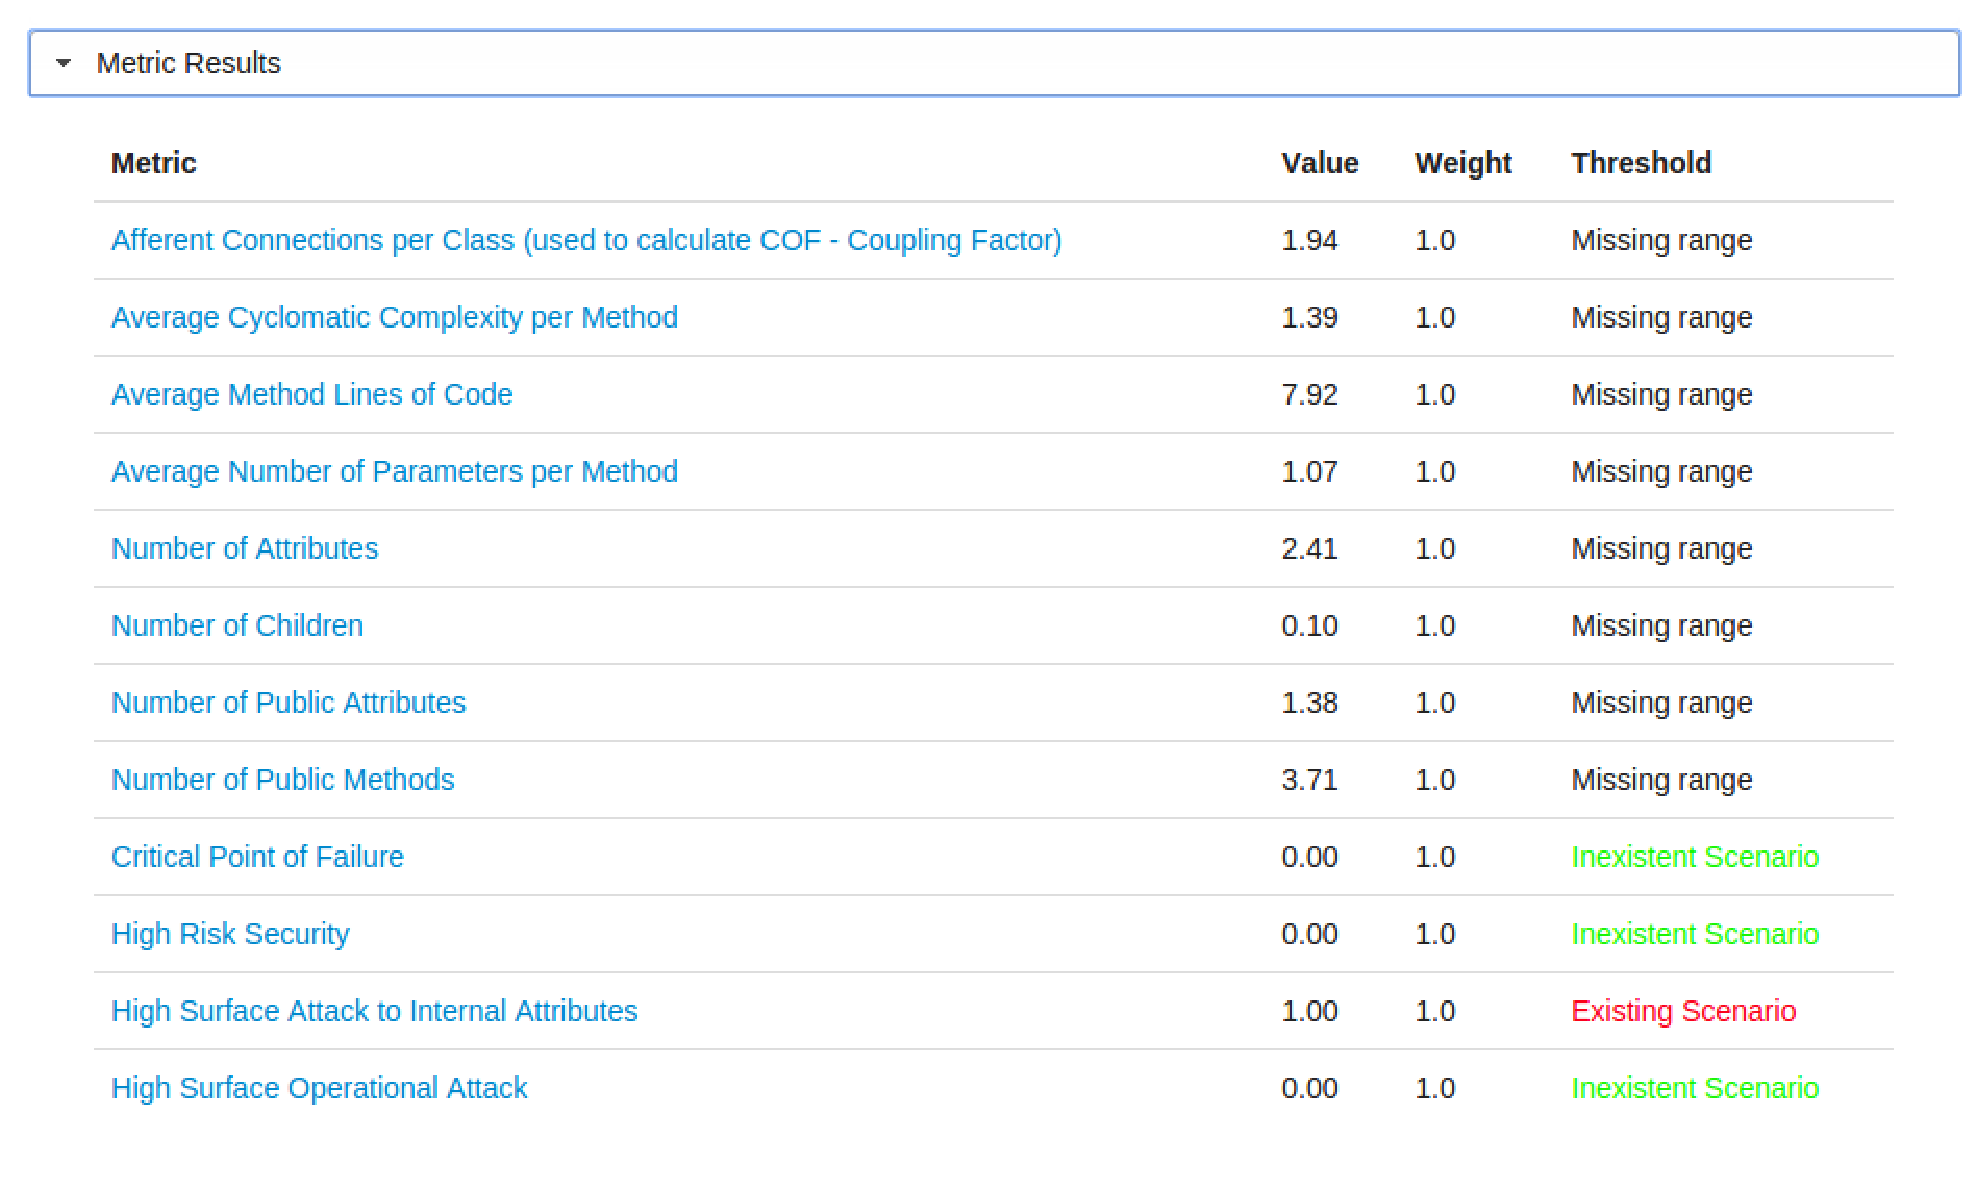
\includegraphics[scale=0.5]{figuras/metrics_info}
		\caption{Apresentação das medições do Mezuro}
		\label{metrics_info}
\end{figure}

No Mezuro, o conceito de agregação é aplicado nas métricas básicas, mas não nas métricas compostas. Na visualização de um pacote (root, da Figura \ref{modules_info}), os valores das métricas básicas são agregadas de acordo com a escolha feita na criação de cada uma (média, mediana, desvio padrão, máximo e mínimo). Entretanto, as métricas compostas, como não possuem agregação, são calculadas sobre os valores agregados das métricas bases que elas utilizam. Para os Cenários de Decisões esta característica não é muito interessante uma vez que pode apresentar falsos negativos. Como exemplo, se o valor agregado das métricas básicas utilizadas por um cenário não corresponderem à existência do cenário, na visualização geral será informado que o cenário não existe, enquanto na verdade ele pode existir em alguns poucos módulos do software. 

Por outro lado, como pode ser observado na Figura \ref{metrics_info}, o cenário Alta Superfície de Ataque a Atributos Internos é o único que é apresentado como existente no projeto, pois as métricas de Atributos Públicos tiveram uma média alta. Nesse sentido, esse cenário deve ser recorrente no projeto e deve ser o foco de melhorias futuras, uma vez que deve se repetir em várias classes. Entretanto, para esse tipo de análise, seria mais interessante ter-se utilizado a agregação por mediana nas métricas básicas, identificando mais adequadamente se os cenários ocorrem na maior parte das classes.

O mais adequado seria o Mezuro apresentar quantas ocorrências do cenário existem para um pacote, ou seja, as métricas compostas terem suas próprias agregações do tipo SOMA. Alguns passos foram dados no contexto do presente trabalho, onde implementamos o suporte à esse tipo de agregação dentro do Kalibro Processor. 

\begin{figure}
	\centering
	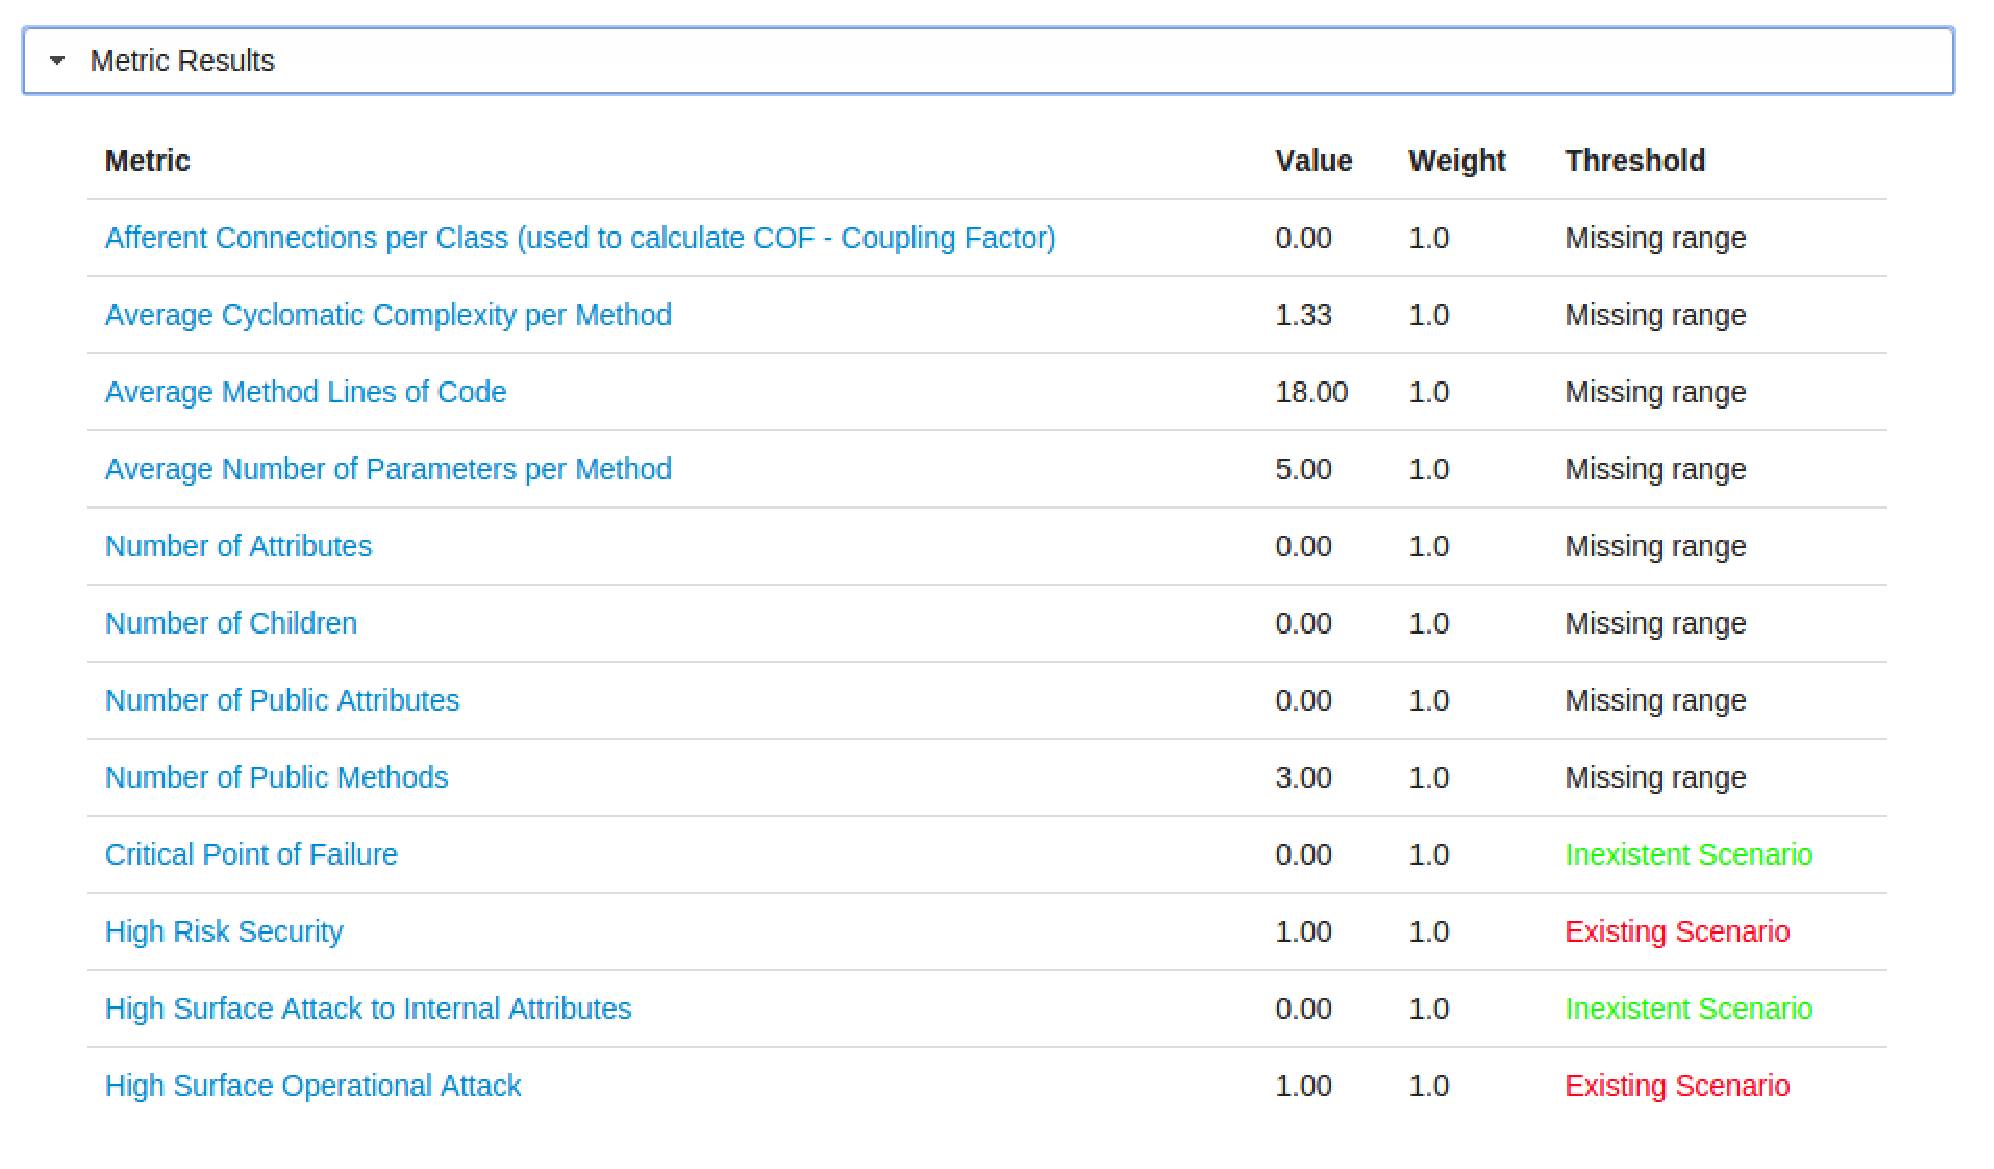
\includegraphics[scale=0.5]{figuras/message_box_class}
	\caption{Resultado da classe MessageBox do projeto Athom Shell}
	\label{message_box_class}
\end{figure}

A visualização da ocorrência dos cenários dentro de cada classe se torna bem interessante. A Figura \ref{message_box_class} apresenta os resultados da classe MessageBox do projeto Athom Shell, avaliado a partir da configuração de cenários criados. O principal foco dos resultados está nos cenários, onde é possível observar claramente que essa classe possui os cenários Risco Elevado de Segurança e Alta Superfície de Ataque Operacional. Além disso, pode-se ainda observar os valores reais obtidos por cada métrica básica para as quais não são providas nenhuma interpretação, uma vez que o foco interpretativo deve estar na natureza do cenário. Pode-se observar ainda que outros dois cenários não caracterizam essa classe.



\subsection{Visualização no DWing}
\label{vision-dw}

A visualização dos cenários no \emph{DWing} é feita com o uso do plugin \emph{Saiku Analytics} disponível na ferramenta \emph{BI server}. Para utilizar o \emph{Saiku Analytics}, depois de logado no \emph{BI server}, deve-se clicar na opção \emph{Create New} -> \emph{New Saiku Analytics}. O \emph{Saiku Analytics} permite o acesso a um cubo de dados publicado e a realização de consultas OLAP em cima dos dados de maneira bem intuitiva, ou , pela criação de \emph{querys} MDX
\footnote{O MDX (\emph{Multidimensional Expression}) é uma linguagem que foi criada com o propósito de manipular dados Multidemensionals. Possui uma sintaxe semelhante ao SQL}
. 

\begin{figure}[H]
	\centering
	\includegraphics[scale=0.3]{figuras/dw-workspace-biserver}
	\caption{Workspace do plugin \emph{Saiku Analytics} no BI server}
	\label{dw-workspace-biserver}
\end{figure}


Na Figura \ref{dw-workspace-biserver} podemos ver a área de trabalho do \emph{Saiku Analytics}. Na área demarcada como 1, podemos escolher os cubos que serão analisados. Na área demarcada como 2, é onde podemos ver as dimensões e medidas do cubo escolhido. Ali podemos ver todos os atributos de cada dimensão. É nessa área que selecionamos quais atributos deverão ver no relatório disposto na área 3. Na área 3 é apresentado o relatório, que é totalmente customizado de acordo com a maneira que os atributos são colocados nos campos "Colunas", "Linhas" e "Filtros".


Para gerar um relatório deve haver pelo menos uma medida envolvida. A partir disso, basta o usuário escolher quais atributos ele quer visualizar, selecionando-os na área 2 e arrastando para os campos "Colunas", "Linhas" e "Filtros" na área 3.



\begin{figure}[H]
	\centering
	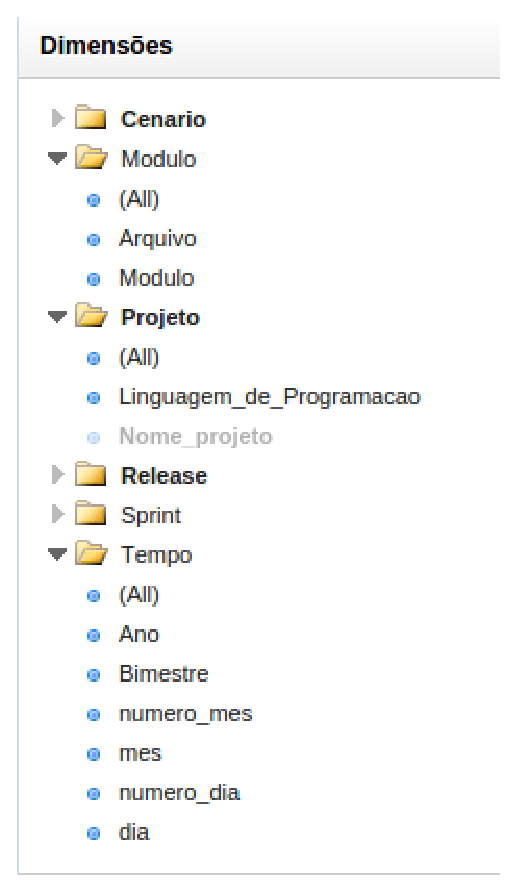
\includegraphics[scale=0.6]{figuras/dw-hierarquias}
	\caption{Atributos que forma as hierarquias para fazer agregações de dados.}
	\label{dw-hierarquias}
\end{figure}

Os atributos das dimensões são mostrados de maneira hierárquica em relação a granularidade, sendo que o primeiro atributo mostrado detém menor nível de detalhe e o ultimo atributo mostrado detém o maior nível de detalhe. Na Figura \ref{dw-hierarquias} podemos ver a hierarquia da dimensão tempo, que possui vários níveis de detalhe. Porém, existem também dimensões que possuem relações hierárquicas, como a dimensão projeto e a dimensão modulo. Isso permite que eu possa analisar os cenários a nível de projeto (mais alto nível) ou a nível de classe , ou arquivo (mais baixo nível), trazendo mais nível de detalhe. As hierarquias são importantes pois os dados podem ser mostrados de forma agregada dependendo do nível de detalhe desejado.


A primeira vista, podemos na Figura \ref{dw-workspace-biserver} que foram encontrados muitos cenários nos projetos. Como os projetos possuem muitas classes e arquivos e que também existem muitas bibliotecas utilizadas e também um framework por parte do \emph{synegy}, gerar um relatório a nível de classe não seria muito interessante, pois este ficaria muito grande. Nesse sentido, as operações OLAP de \emph{Slice and Dice} podem ser feitas através dos filtros. Isso permite que sejam selecionados os dados de apenas uma release específica, como também classes específicas, arquivos específicos. Permite também analisar apenas os dados relativos a um tipo de cenário. Enfim, com os filtros, diferentes inúmeras consultas podem ser feitos e relatórios de diversas naturezas podem ser gerados.


\begin{figure}[H]
	\centering
	\includegraphics[scale=0.3]{figuras/dw-graficos-cenarios}
	\caption{Gráfico gerado pelo \emph{Saiku Analytics} que permite ver a quantidade de cenários de decisões ao logo de cada release}
	\label{dw-graficos-cenarios}
\end{figure}

Outra funcionalidade interessante é a possibilidade de geração de gráficos a partir do relatório criado. Na Figura \ref{dw-graficos-cenarios} podemos ver o comportamento da quantidade de cenários de decisões encontrados no projeto Octave ao longo de suas releases. 


\begin{figure}[H]
	\centering
	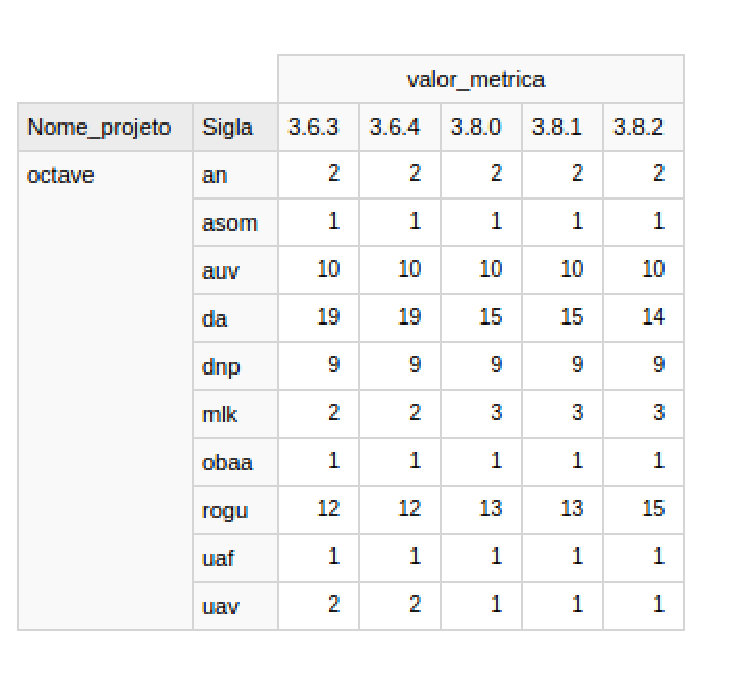
\includegraphics[scale=0.7]{figuras/dw-relatorio-octave}
	\caption{Relatório com a quantidade de vulnerabilidades por release e por tipo de vulnerabilidade específica encontradas no Octave}
	\label{dw-relatorio-octave}
\end{figure}

\begin{figure}[H]
	\centering
	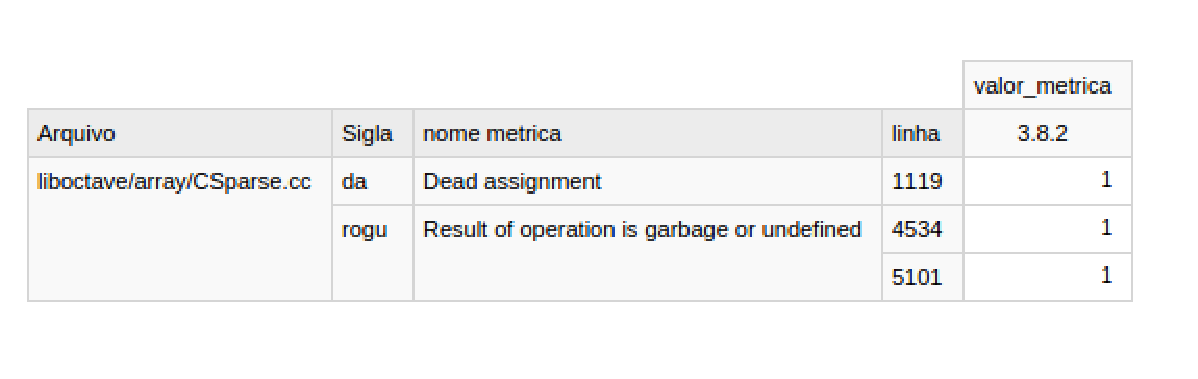
\includegraphics[scale=0.7]{figuras/dw-sec-octave}
	\caption{Relatório que verifica quais as vulnerabilidades foram encontradas no arquivo \emph{CSparse.cc}, indicando também a linha de ocorrência}
	\label{dw-sec-octave}
\end{figure}

As mesmas operações e manipulações dos dados podem ser feitas no cubo que armazena as métricas de segurança. Como a natureza das métricas de vulnerabilidades é contar a quantidade de ocorrências de uma vulnerabilidades específica, esse tipo de métrica pode ser agregada com a operação de soma. Dessa forma, podemos ver o total de vulnerabilidades existente no projeto. A Figura \ref{dw-relatorio-octave} mostra o relatório com o total de vulnerabilidades de cada tipo encontradas nas releases do Octave observadas. Realizando operações de \emph{Drill down}, podemos chegar até na linha que foi encontrada uma vulnerabilidade específica, como mostrado na Figura \ref{dw-sec-octave}. Isso é bom pois é apontado o local que se encontra a vulnerabilidade e que deve ser refatorado. Não foram encontradas vulnerabilidades específicas no Synergy, apenas no Octave.


\subsection{Análise e Discussão}
\label{ana-disc}

Os dois estudos de casos desenvolvidos no contexto deste trabalho tiverem como objetivo representar os Cenários de Decisões em ferramentas de tomada de decisão. O primeiro estudo foi baseado no projeto Mezuro, enquanto o segundo foi baseado em um ambiente DWing para os quais a mesma metodologia de desenvolvimento de estudo de caso foi aplicada. 

O Mezuro, sendo uma plataforma já utilizada para monitoramento de projetos livres, foi adaptada para suportar os cenários a partir da evolução das métricas compostas, funcionalidade já existente no Mezuro. Esta evolução se apresentou como uma boa opção dado o tempo e complexidade de se implementar uma estrutura completa de Cenário de Decisão na ferramenta. Além disso, as métricas compostas contém informações fundamentais para a identificação e descrição dos cenários, além de oferecer o recurso de criação de \emph{scripts} para definição dos cenários.

Algumas contribuições técnicas puderam ser feitas à plataforma Mezuro. É importante enfatizar que as evoluções propostas à plataforma sempre foram discutidas e adaptadas com a comunidade de desenvolvedores. Neste sentido, alinhou-se as necessidade deste trabalho às expectativas de melhorias na comunidade.

No Mezuro, a criação de configurações e o monitoramento de projetos pode ser realizado com passos simples, comparado aos passos necessários para reprodução no DW. Da mesma forma, o Mezuro visa oferecer uma interface simples para apresentação dos resultados de medições, oferecendo navegabilidade entre os módulos do software, agregação de valores de métricas e interpretações qualitativas para as métricas.

Entretanto, o fato de não existir agregação para métricas compostas limita a visualização de cenários a nível de pacotes e projetos, uma vez que pode dar margem à erros interpretativos e dificulta um planejamento a partir de uma visão geral sobre o projeto. Por outro lado, a visualização da cenários dentro das classes é simples, completa e informativa, apoiando a tomada de decisões, principalmente para os desenvolvedores, uma vez que o nível de granularidade é menor.

Foi possível representar todos os Cenários de Design Seguro para C++ dentro do Mezuro através de uma configuração que pode ser utilizada por qualquer projeto em C++ que venha a ser avaliado através do Mezuro. Essa configuração é uma contribuição técnica para a plataforma, provida dos estudos realizados nesta monografia. Por outro lado, devido aos problemas já relatados sobre o Analizo, não foi possível utilizar métricas de vulnerabilidades no Mezuro para a construção de novos cenários.

Por fim, vale ressaltar que o recurso de análise periódica oferecida pela plataforma complementa a interpretação através de Cenários de Decisões, podendo apoiar o desenvolvimento e evolução do software diariamente.

Embora o \emph{DWing} seja uma solução de construção mais complexa em relação Mezuro, ele mostrou-se uma abordagem interessante e eficiente para monitorar a ocorrência de cenários de decisões em um projeto de software. O principal destaque está no caráter temporal de análise dos dados, ou seja, no \emph{DWing} é possível armazenar os dados coletados ao longo do tempo, permitindo uma perspectiva sobre o projeto no que diz repeito a saber se está havendo melhoria ou não da qualidade desse software, que no caso deste trabalho o foco foi em características de \emph{design} seguro. Com esse tipo de análise, alinhado com as atividades de desenvolvimento, o Engenheiro de Software pode identificar quais práticas de desenvolvimento estão dando resultado em relação a melhoria da segurança do código, ou quais não estão. Além disso, a solução ajuda na identificação do local onde deve ser feita melhorias e também auxilia na identificação de quais práticas precisam ser melhoradas na equipe por conta do perfil dos cenários mais encontrados.

Diferente do Mezuro, foi possível realizar agregações e também reproduzir todos os cenários propostos. Isso se deu por conta de que não se tratou da evolução de uma ferramenta que já possui suas limitações, mas sim da construção de um ambiente completo que atendesse as necessidades desejadas.

Porém, como já discutido, o \emph{DWing} é uma solução complexa de se construir, principalmente no que se diz respeito aos  mecanismos de ETL dos dados. Outro aspecto negativo foi que, nesta monografia, não conseguimos automatizar completamente a carga de dados no ambiente, fazendo com que seja necessário ter os relatórios das ferramentas em mão para então poder realizar a coleta de dados, tarefa que é feita de forma automática pelo Mezuro graças ao Kalibro Processor. A total automatização do ambiente só se daria com a criação de shellscripts e utilização de Jobs no PDI.


Por fim, nota-se que as duas soluções realizam os mesmos passos na coleta e tratamento dos dados medidos, tendo-se uma redundância entre elas. Uma opção seria utilizar o Mezuro como a principal fonte de dados para o DWing, dado que a coleta de dados do Mezuro já é estável e mantida por uma comunidade de desenvolvedores.